\chapter[\textit{iFlow}]{\textit{iFlow}}

\label{chap:proposta}

Este capítulo visa detalhar o \textit{iFlow}, o qual é uma ferramenta que se baseia no processo proposto pela Engenharia de Requisitos para gerenciar e dar suporte àqueles que estão inseridos nesse contexto. Primeiramente, tem-se uma seção apresentando a contextualização do \textit{iFlow} (Seção \ref{sec:contextualizacao}). Em seguida, apresenta-se a ferramenta \textit{iFlow} (Seção \ref{sec:sobre_a_ferramenta}). Adicionalmente, descreve-se a arquitetura de \textit{software} (Seção \ref{sec:arquitetura_da_solucao}), utilizada para o desenvolvimento da ferramenta, além das especificidades dos módulos do sistema, seguindo para a apresentação da identidade visual (Seção \ref{sec:identidade_visual}). Logo depois, apresentam-se os principais diagramas da ferramenta (Seção \ref{sec:diagramas_da_aplicacao}). Posteriormente, tem-se a apresentação das telas desenvolvidas do \textit{iFlow} e do \textit{backlog} da ferramenta (seções \ref{sec:prototipo_de_alta_fidelidade} e \ref{sec:backlog_do_produto}). Por fim, têm-se as telas desenvolvidas do \textit{iFlow} e o resumo do capítulo (Seção \ref{sec:versao_final_iFlow} e \ref{sec:resumo_proposta}).

\section{Contextualização}

\label{sec:contextualizacao}

A principal justificativa para o desenvolvimento da ferramenta \textit{iFlow} diz respeito a buscar minimizar e evidenciar os problemas associados aos processos da Engenharia de Requisitos. Vale ressaltar, que não existem, até o momento da publicação deste Trabalho de Conclusão de Curso, trabalhos correlatos que tenham o escopo de atuação e busquem solucionar os problemas da área da forma proposta.

Reproduzindo um papel essencial no desenvolvimento de produtos de \textit{software}, a Engenharia de Requisitos fornece uma maneira de entender e descrever problemas que precisam de uma solução de \textit{software}. Além disso, é um ramo que está inteiramente ligado ao ciclo de desenvolvimento do \textit{software} \cite{elliott2012software}. Dessa forma, por se tratar de uma área negligenciada por muitos, foi realizada a construção de uma ferramenta que oferece apoio tecnológico, viabiliza e semi-automatiza as etapas da Engenharia de Requisitos, com o propósito de facilitar e melhorar estes processos.

A seguir, tem-se uma descrição mais aprofundada da ferramenta desenvolvida neste Trabalho de Conclusão de Curso.

\section{Sobre a Ferramenta \textit{iFlow}}

\label{sec:sobre_a_ferramenta}

A ferramenta \textit{iFlow} tem o objetivo de viabilizar e semi-automatizar o processo da Engenharia de Requisitos, de modo a embasar a construção de um produto de \textit{software} e evitar que retrabalhos e desperdícios de tempo ocorram devido ao mau planejamento. Neste sentido, algumas automatizações foram realizadas, de modo a estabelecer e se apoiar no conceito de um \textit{Minimum Viable Product} (MVP). Além disso, a ferramenta confere ênfase às etapas da Engenharia de Requisitos. Dessa forma, a ferramenta é composta por algumas etapas, dentre elas: 
% Verificar isso aqui amanhã %
a) pré-rastreabilidade; b) elicitação; c) modelagem; d) \textit{house of quality}; e e) pós-rastreabilidade. 

\subsection{Pré-rastreabilidade}

Nesta primeira etapa, o foco da ferramenta foi em aplicar os conceitos propostos em pré-rastreabilidade (Seção \ref{sec:pre-rastreabilidade}), e iniciar o processo da Engenharia de Requisitos, descrevendo as primeiras definições do produto de \textit{software} em questão, iniciando o levantamento dos requisitos.

Com esse objetivo, os artefatos usados para esta etapa são o \textit{5W2H} (Seção \ref{sec:5w2h}), que sintetiza a ideia inicial do produto, e o \textit{Rich Picture} (Seção \ref{sec:rich_picture}), que transcreve visualmente os atores e o fluxo de informações envolvidos no processo.

\subsection{Elicitação}

\label{sec:proc_elicitacao}

Estabelecida a visão geral do produto de \textit{software}, a ferramenta parte para a segunda etapa do processo, que levanta o maior número possível de requisitos. A intenção é que se colete diferentes pontos de vistas em diferentes contextos e com opiniões distintas, visando a aquisição de definições do produto mais ricas que agregue mais valor para os \textit{stakeholders}.

Dessa forma, na ferramenta, existem diversas propostas de métodos que proporcionam modelos que auxiliam na elicitação dessas funcionalidades. Vale salientar que tais métodos não são obrigatórios para que o usuário siga para a próxima etapa, mas evidencia-se a importância desta etapa, além de uma confirmação de que as funcionalidades levantadas são suficientes para a construção do produto de \textit{software}.

No contexto de cada ferramental, o usuário tem a possibilidade de adicionar diferentes fontes de dados para compor o artefato, sendo: imagens, áudios e documentos de texto. O intuito é que, a partir dessas informações, novas funcionalidades sejam adquiridas.

% REVISAR

% Por conta da complexidade de cada artefato, são disponibilizadas definições rápidas, cujos objetivos são guiar e conduzir de maneira mais adequada o desenvolvimento. Para estudos mais aprofundados, fontes da literatura reconhecidas são sugeridas na ferramenta.

Neste sentido, os artefatos disponibilizados para viabilizar a etapa da elicitação são:

\begin{itemize}
    \item \textit{Brainstorming} (Seção \ref{sec:brainstorming}), que coleta o maior número de ideias acerca do produto de \textit{software};
    \item Questionário (Seção \ref{sec:questionario}), que tem o objetivo de coletar o maior número de informações a respeito do tema em questão;
    \item Protótipo de Baixa Fidelidade (\ref{sec:prototipo-def}), que ajuda, visualmente, na elicitação dos requisitos;
    \item \textit{Storytelling} (Seção \ref{sec:storytelling}), que extrai as \textit{features} do sistema em um determinado contexto;
    \item Entrevista (Seção \ref{sec:entrevista}), que, de certa forma, traz uma visão mais concreta acerca de um tema pelo fato de se ter uma comunicação mais natural entre os envolvidos, e
    \item Análise de Protocolo (Seção \ref{sec:analise-protocolo}), que sintetiza os pensamentos de um usuário e, a partir disso, tem-se a extração de possíveis requisitos do sistema.
\end{itemize}

\subsection{Modelagem}

\label{sec:modelagem_proposta}

Com as funcionalidades levantadas, a ferramenta segue para a próxima etapa do processo, que visa colocar em modelos estruturados todas as ideias obtidas na etapa anterior (Seção \ref{sec:proc_elicitacao}). Diferentemente da elicitação, que tem uma visão muito aberta e livre para proporcionar um espaço saudável para que a criatividade seja o principal foco, este nível visa chegar em um ponto mais concreto e consistente para a construção de uma aplicação. O propósito, é gerar modelos capazes de representar características ou comportamentos do produto de \textit{software}, que possam guiar todo o processo de desenvolvimento.

Vale destacar a importância deste processo, pois concluída esta etapa, o usuário deve viabilizar uma forma para a construção do produto de \textit{software}. Neste ponto, deve-se ter uma visão mais concreta e definitiva da aplicação que se almeja desenvolver.

Esta etapa é imprescindível, pois aqui são gerados artefatos essenciais para a aplicação que será desenvolvida. Sendo assim, os artefatos usados para esta etapa são o \textit{Backlog} (Seção \ref{sec:backlog}), que concentra a lista de defeitos, melhorias solicitadas pelo cliente, funcionalidades, entre outros itens que expressam os requisitos do produto; o NFR \textit{Framework} (Seção \ref{sec:nfr}), que sintetiza os requisitos não funcionais do sistema no formato de um grafo, e os Léxicos (\ref{sec:lexicos}), que transcrevem todos os vocábulos utilizados no domínio de uma aplicação.

% \subsection{Verificação}

% Para evitar retrabalhos e gerar artefatos que estejam os mais corretos e concisos possíveis, esta etapa tem o objetivo de revisar o que foi gerado até o momento (Seção \ref{sec:verificacao}). No contexto de cada artefato, existem regras e métodos que devem ser seguidos ou algum objetivo que existe ao realizar aquela atividade. Portanto, para cada um dos artefatos gerados, a ferramenta sugere alguns pontos de checagem para que o usuário revise aquilo que foi elaborado, como propõe \citeauthoronline{design_fagan} (\citeyear{design_fagan}) em seu método de inspeção. Todavia, isso não impede que o usuário defina pontos que ache relevante de avaliar.

% Definidos quais pontos são relevantes para a avaliação, o usuário dispõe de uma visualização conjunta do artefato revisado para poder realizar o processo de \textit{inspeção}. Feito isso, a ferramenta apresenta ao usuário métricas de precisão do artefato, viabilizando uma correção dos pontos de melhoria levantados.

% \subsection{Pós-rastreabilidade}

% Em posse de requisitos modelados e concisos, esta etapa trata de um processo, automático gerado pela ferramenta, que produz um grafo (Seção \ref{sec:grafos}) a partir do que foi realizado nas etapas anteriores. Esse artefato, chamado \textit{Backward-from} (Seção \ref{sec:pos-rastreabilidade}), mantém um requisito desde sua origem, e mantém a visão obtida no momento que o requisito foi extraído.

\subsection{Priorização}
% REVISAR

Essa etapa é de suma importância dentro do contexto de Engenharia de Requisitos, pois nela que é definido o Produto Mínimo Viável (Seção \ref{sec:priorizacao}) a partir da \textit{House of Quality} (Seção \ref{sec:house_of_quality}), onde se tem a correlação dos requisitos funcionais e não funcionais e seus \textit{softgoals}. Aqui, determina-se quais são as principais funcionalidades do produto de \textit{software}, que devem ser validadas e efetivadas pelo usuário final. Dessa forma, para a geração do Produto Mínimo Viável, faz-se o uso de Grafos (Seção \ref{sec:grafos}), utilizando-se de um algoritmo de Menor Caminho (Dijkstra).

\section{Arquitetura da Ferramenta \textit{iFlow}}

\label{sec:arquitetura_da_solucao}

Conforme é observado na Figura \ref{fig:arquitetura}, a arquitetura de \textit{software} do \textit{iFlow} inclui a integração de dois módulos: o \textit{front-end} e o \textit{back-end}.

\begin{figure}[]
    \begin{center}
        \caption{{Arquitetura do \textit{Software} da ferramenta \textit{iFlow}}}
        \label{fig:arquitetura}
        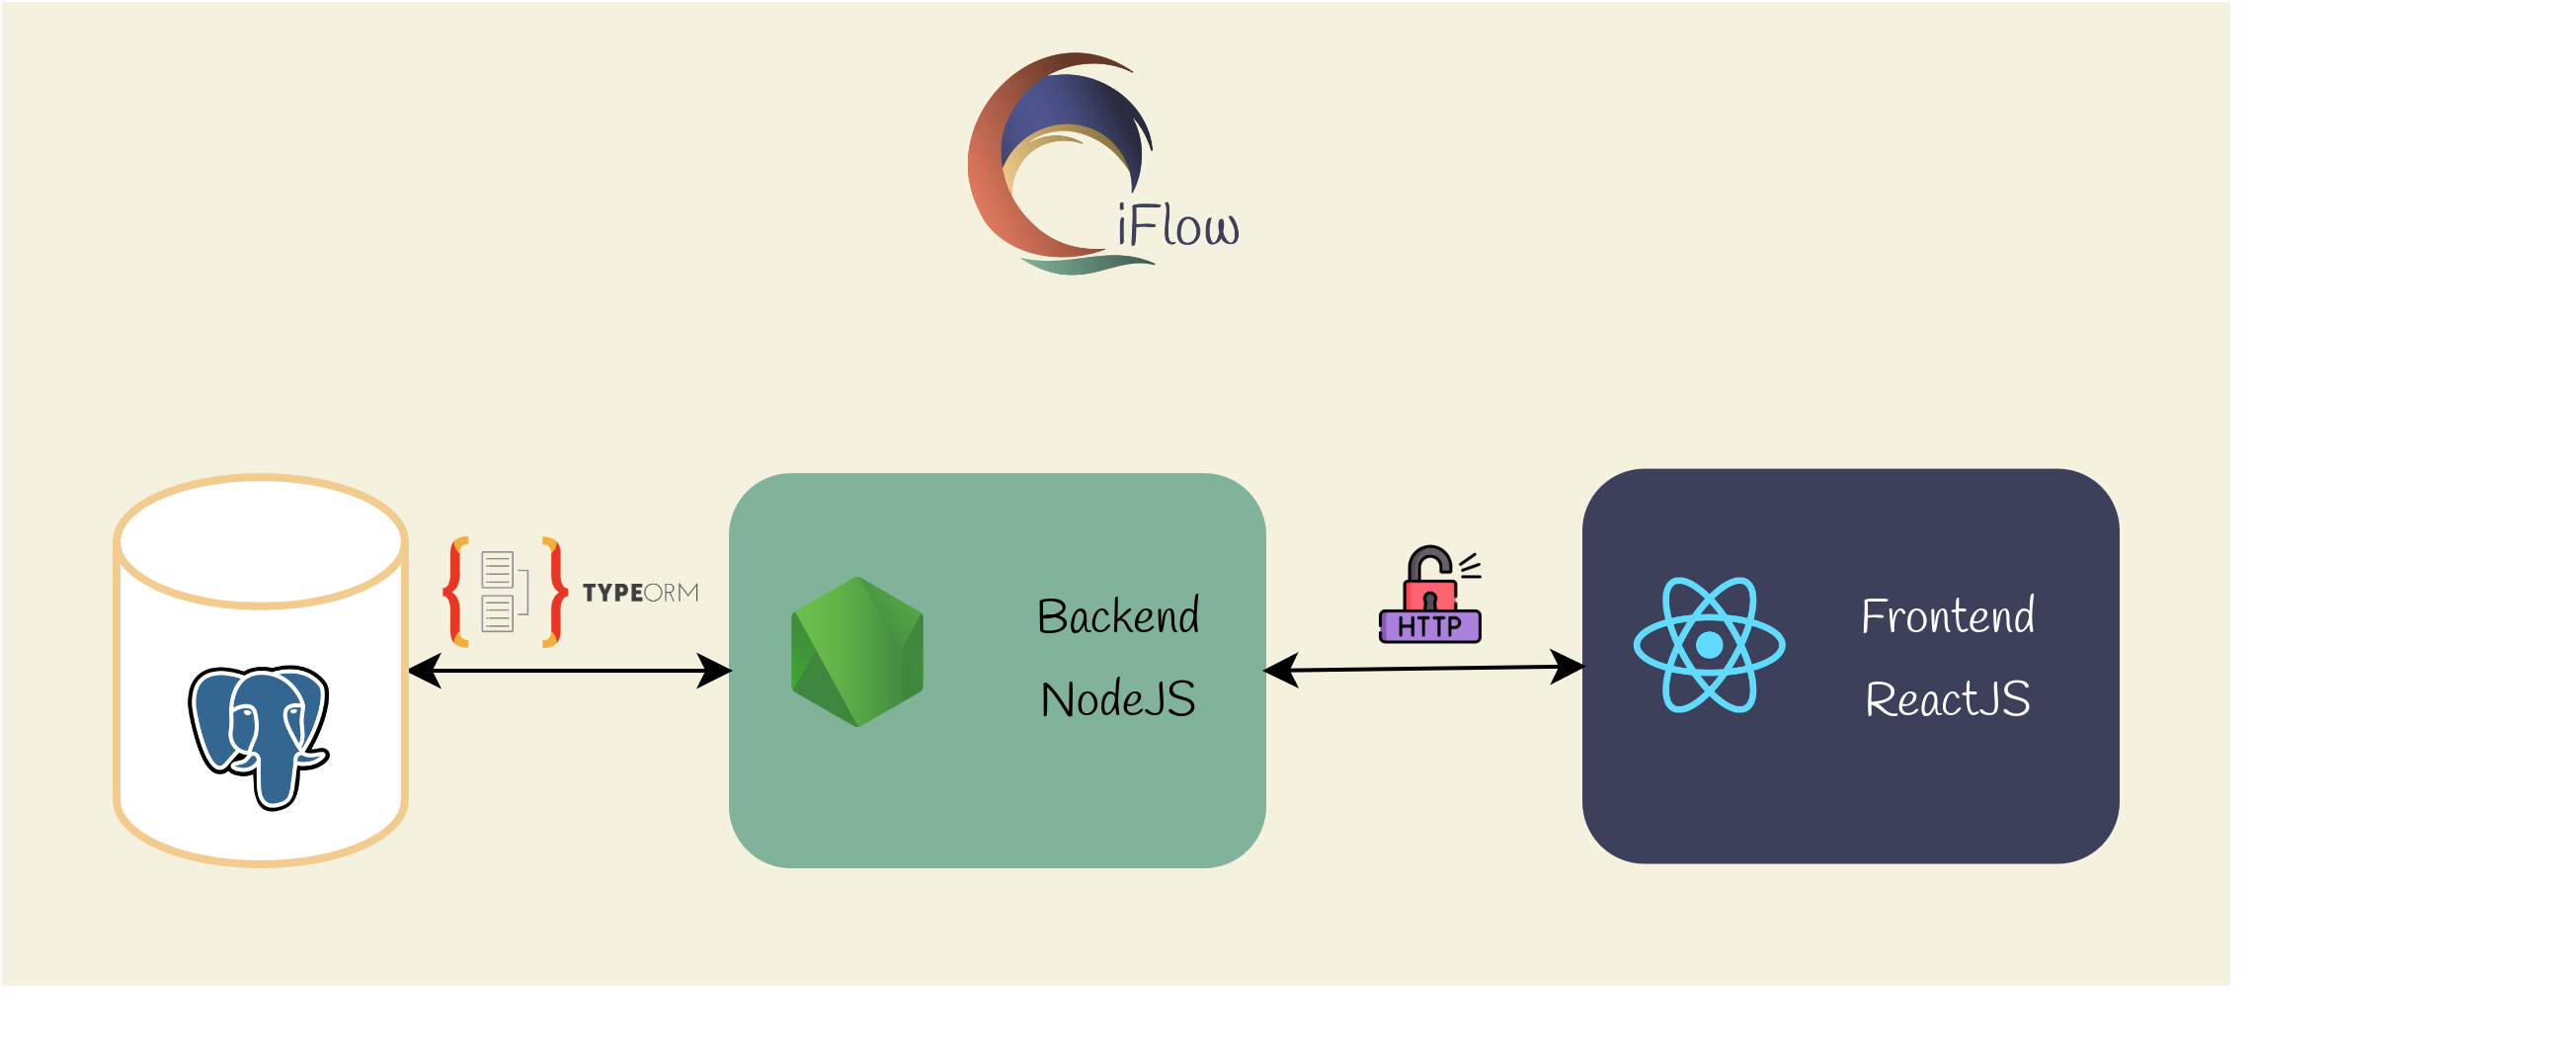
\includegraphics[scale=1.0]{figuras/Proposta/arquitetura.png}
        \legend{Fonte: Autores, 2022.}
    \end{center}
\end{figure}

\subsection{\textit{Front-end}}
O \textit{Front-end} tem a função de realizar as interações com o usuário e com o \textit{back-end}. Além disso, é responsável pela \textit{interface} da ferramenta utilizando recursos \textit{HTML} e \textit{CSS} com o \textit{framework} \textit{React}. Sendo assim, essas tecnologias foram utilizadas devido ao grande suporte que elas oferecem para a construção de \textit{interfaces} de usuário interativas, descritas com mais detalhes no Capítulo \ref{chap:referencial_tecnologico}.

\subsection{\textit{Back-end}}
O \textit{Back-end} tem a função de realizar a conexão com o banco de dados; armazenar os dados que são consumidos ou manipulados pelo \textit{software}, e por realizar o tratamento dos dados. Dessa forma, foi utilizada a tecnologia \textit{Node.js} visando realizar a comunicação entre as camadas de banco de dados e de \textit{front-end}. A tecnologia é descrita com mais detalhes no Capítulo \ref{chap:referencial_tecnologico}.

\section{Identidade Visual da Ferramenta \textit{iFlow}}

\label{sec:identidade_visual}

A Identidade Visual é um conjunto de elementos gráficos e visuais, com o intuito de mostrar os principais elementos do produto e seus valores. Com o intuito de dar uma identidade visual para a ferramenta \textit{iFlow}, foi elaborado um manual que elenca os logotipos, as cores, a tipografia e os símbolos definidos para o projeto. Esse manual está descrito com maiores detalhes no Apêndice \ref{apendice:identidade_visual}.

\subsection{Logotipo}
O logotipo da ferramenta é a representação de ondas buscando transmitir a noção do processo proveniente da Engenharia de Requisitos, conforme pode-se observar na Figura \ref{fig:logotipo}.

\begin{figure}[]
    \begin{center}
        \caption{{Logotipo da Ferramenta \textit{iFlow}}}
        \label{fig:logotipo}
        
\includegraphics[scale=1.0]{figuras/Proposta/logotipo.png}
        \legend{Fonte: Autores, 2022.}
    \end{center}
\end{figure}

\section{Modelagem da Ferramenta \textit{iFlow}}

\label{sec:diagramas_da_aplicacao}

\subsection{Diagramas de Banco de Dados}

Os diagramas de Banco de Dados visam modelar como os dados serão armazenados na Ferramenta \textit{iFlow}. O DER (Figura \ref{fig:diagrama_conceitual}) é a representação gráfica e a principal ferramenta de visualização dos relacionamentos entre as entidades do sistema. Já o DL (Figura \ref{fig:diagrama_logico}) descreve como os dados serão armazenados no banco, além dos seus relacionamentos.

\begin{figure}[]
    \begin{center}
        \caption{{DER do Banco de Dados do \textit{iFlow}}}
        \label{fig:diagrama_conceitual}
        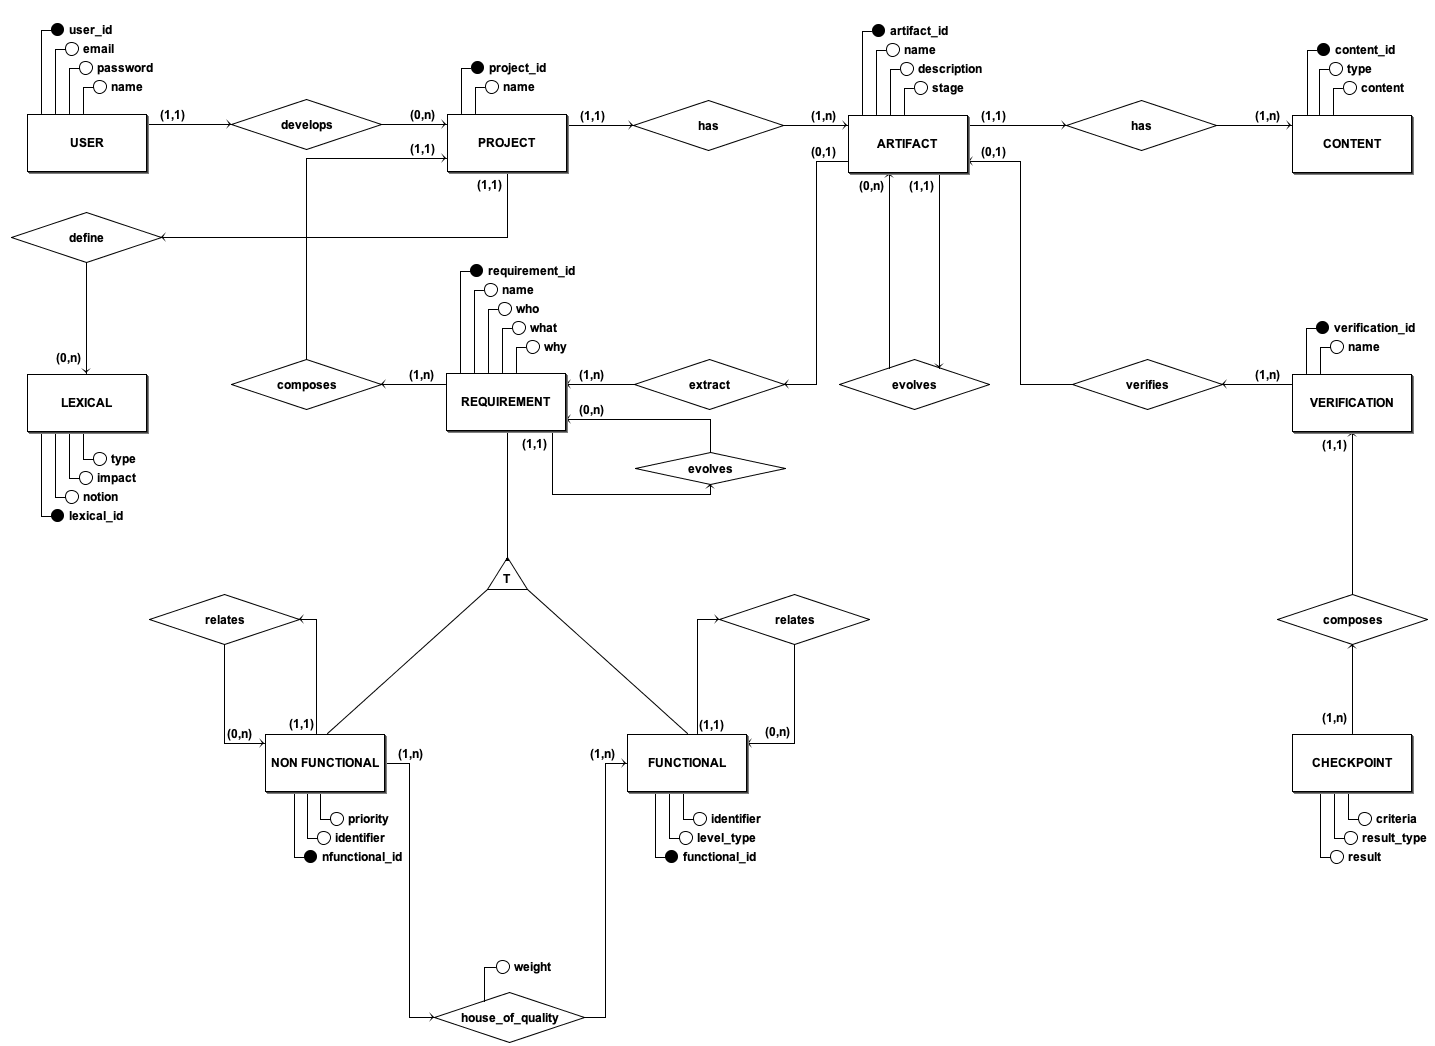
\includegraphics[scale=0.30]{figuras/Proposta/Conceitual_iFlow.png}
        \legend{Fonte: Autores, 2022.}
    \end{center}
\end{figure}

\begin{figure}[]
    \begin{center}
        \caption{{DL do Banco de Dados do \textit{iFlow}}}
        \label{fig:diagrama_logico}
        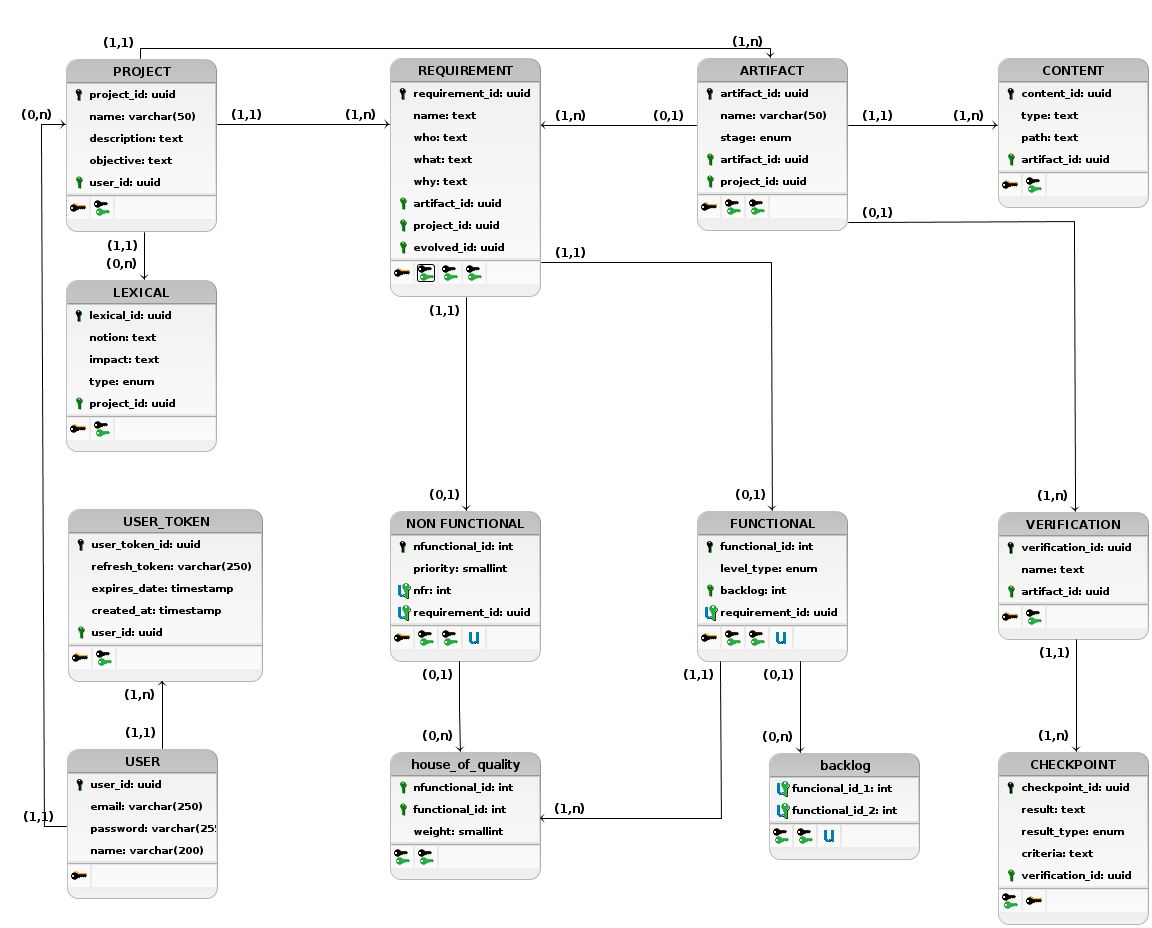
\includegraphics[scale=0.37]{figuras/Proposta/Logico_iFlow.png}
        \legend{Fonte: Autores, 2022.}
    \end{center}
\end{figure}

O código que cria a base de dados da Ferramenta \textit{iFlow} está disponível no Apêndice \ref{ap:db_sql}.

\subsection{Diagrama de Pacotes}

O Diagrama de Pacotes é representado como um esquema estático, possibilitando a visualização e a organização do projeto de maneira mais adequada e simplificada, proporcionando uma visão em módulos, facilitando o entendimento do projeto durante o desenvolvimento e em possíveis manutenções. Foram desenvolvidos a partir das melhores práticas e padrões adotadas por ambas as comunidades, \textit{ReactJS} e \textit{NodeJS}. Dessa forma, os diagramas das Figuras \ref{fig:pacotes_backend} e \ref{fig:pacotes_frontend} procuram detalhar a organização interna dos pacotes, quanto aos diferentes módulos da Ferramenta \textit{iFlow}, \textit{Front-end} e \textit{Back-end}.

Uma visualização ampliada foi adicionada para o detalhamento da pasta do diagrama de pacotes do \textit{Back-end}, na Figura \ref{fig:pacotes_backend_shared}, para melhor visualização.

\begin{figure}[]
    \begin{center}
        \caption{{Diagrama de Pacotes do \textit{Backend} do \textit{iFlow}}}
        \label{fig:pacotes_backend}
        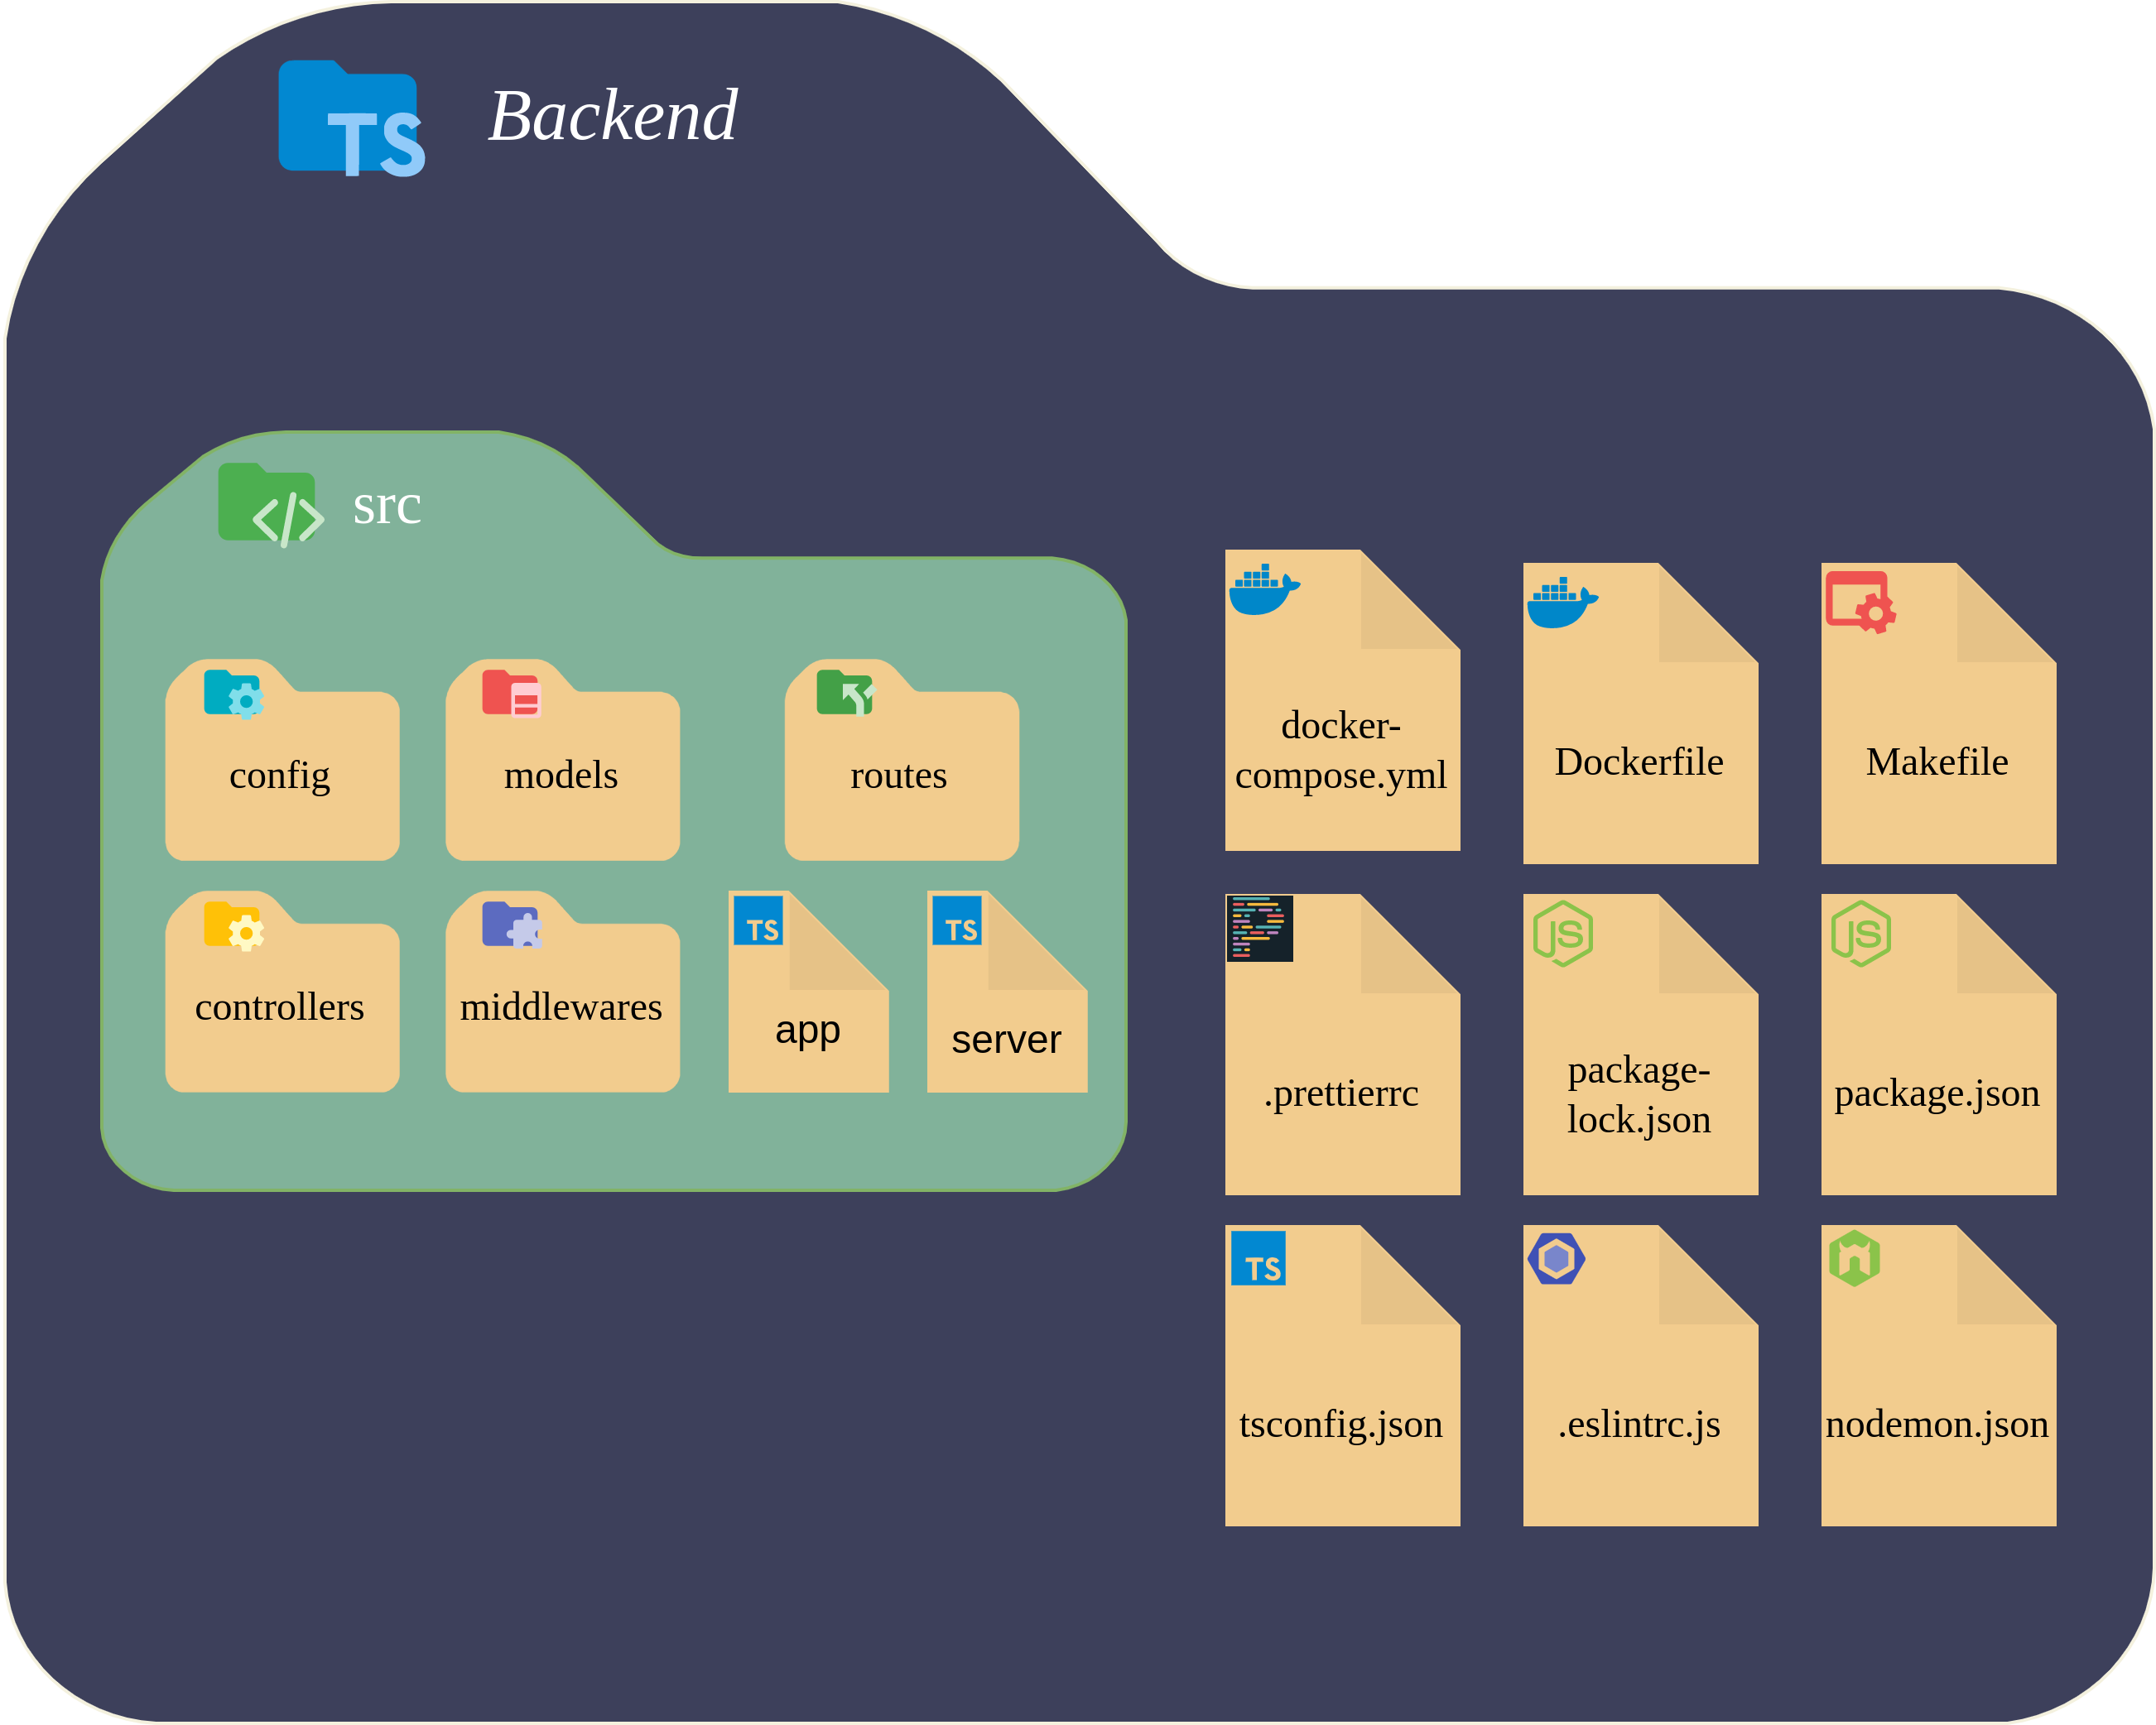
\includegraphics[scale=0.9]{figuras/Proposta/Diagrama_de_Pacotes-Backend.png}
        \legend{Fonte: Autores, 2022.}
    \end{center}
\end{figure}

\begin{figure}[]
    \begin{center}
        \caption{{Diagrama de Pacotes do \textit{Backend} do \textit{iFlow}: detalhamento da pasta \textit{shared}}}
        \label{fig:pacotes_backend_shared}
        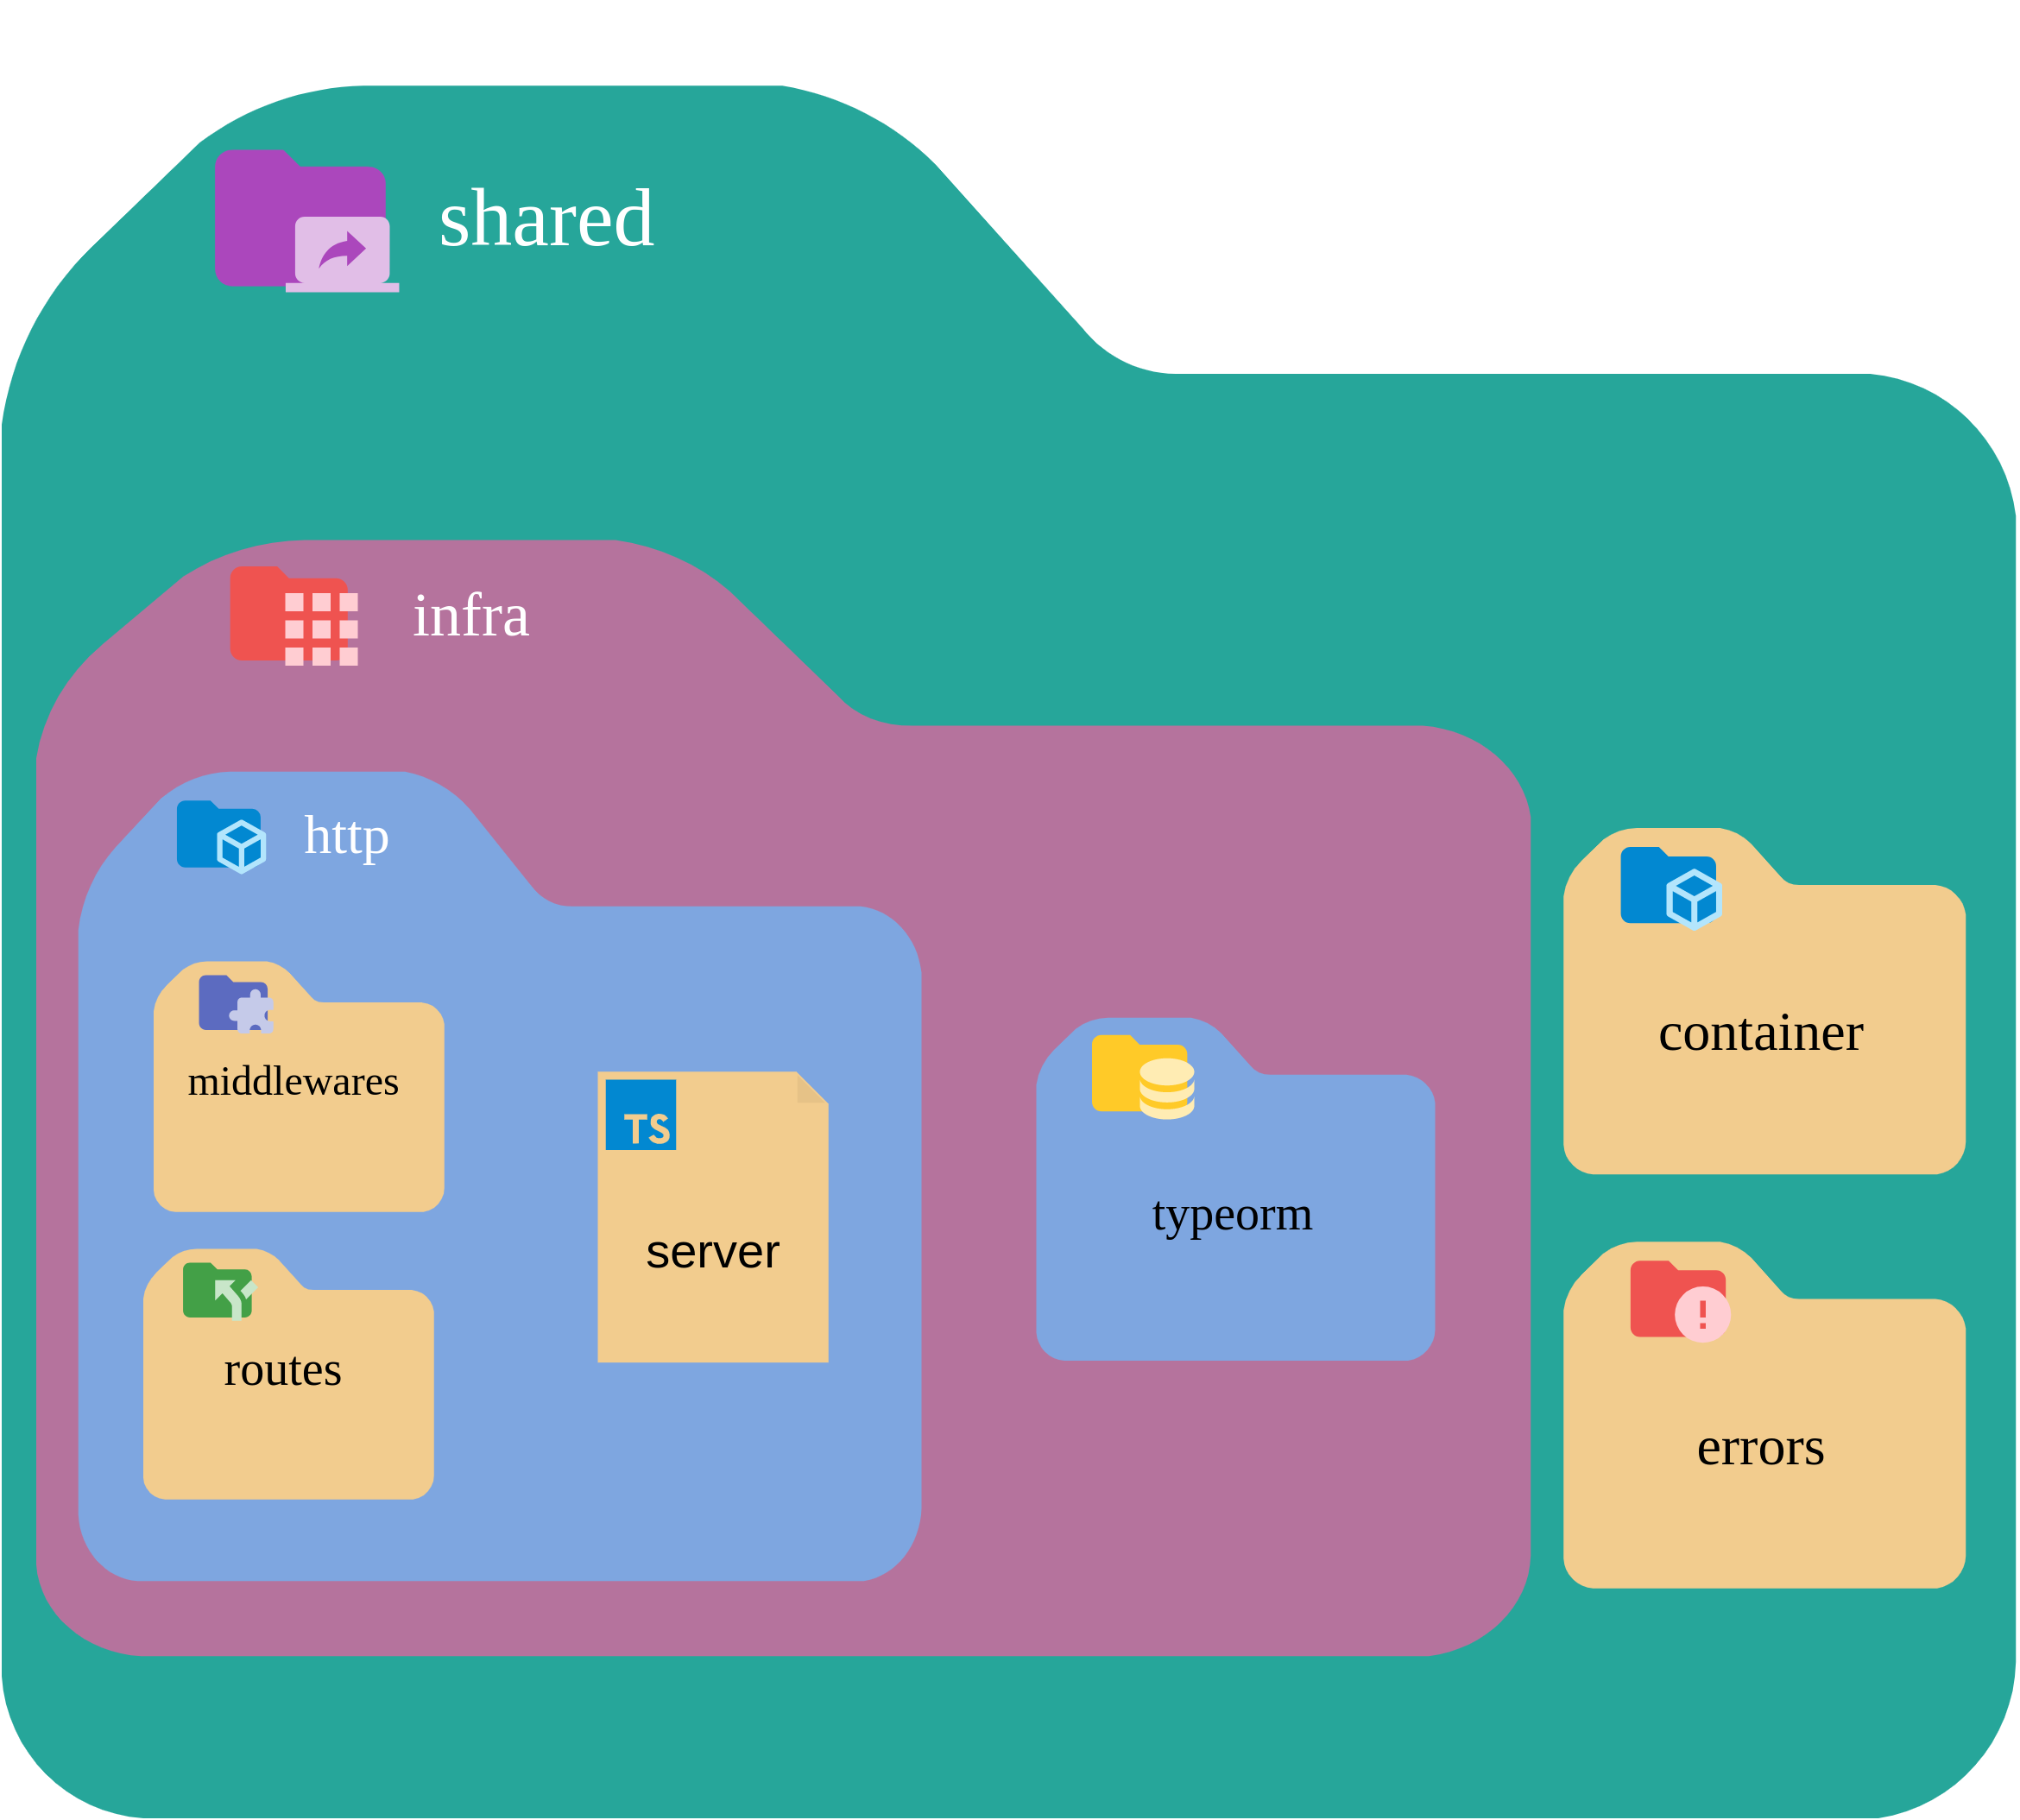
\includegraphics[scale=0.9]{figuras/Proposta/Diagrama_de_Pacotes-Backend_shared.png}
        \legend{Fonte: Autores, 2022.}
    \end{center}
\end{figure}

\begin{figure}[]
    \begin{center}
        \caption{{Diagrama de Pacotes do \textit{Frontend} do \textit{iFlow}}}
        \label{fig:pacotes_frontend}
        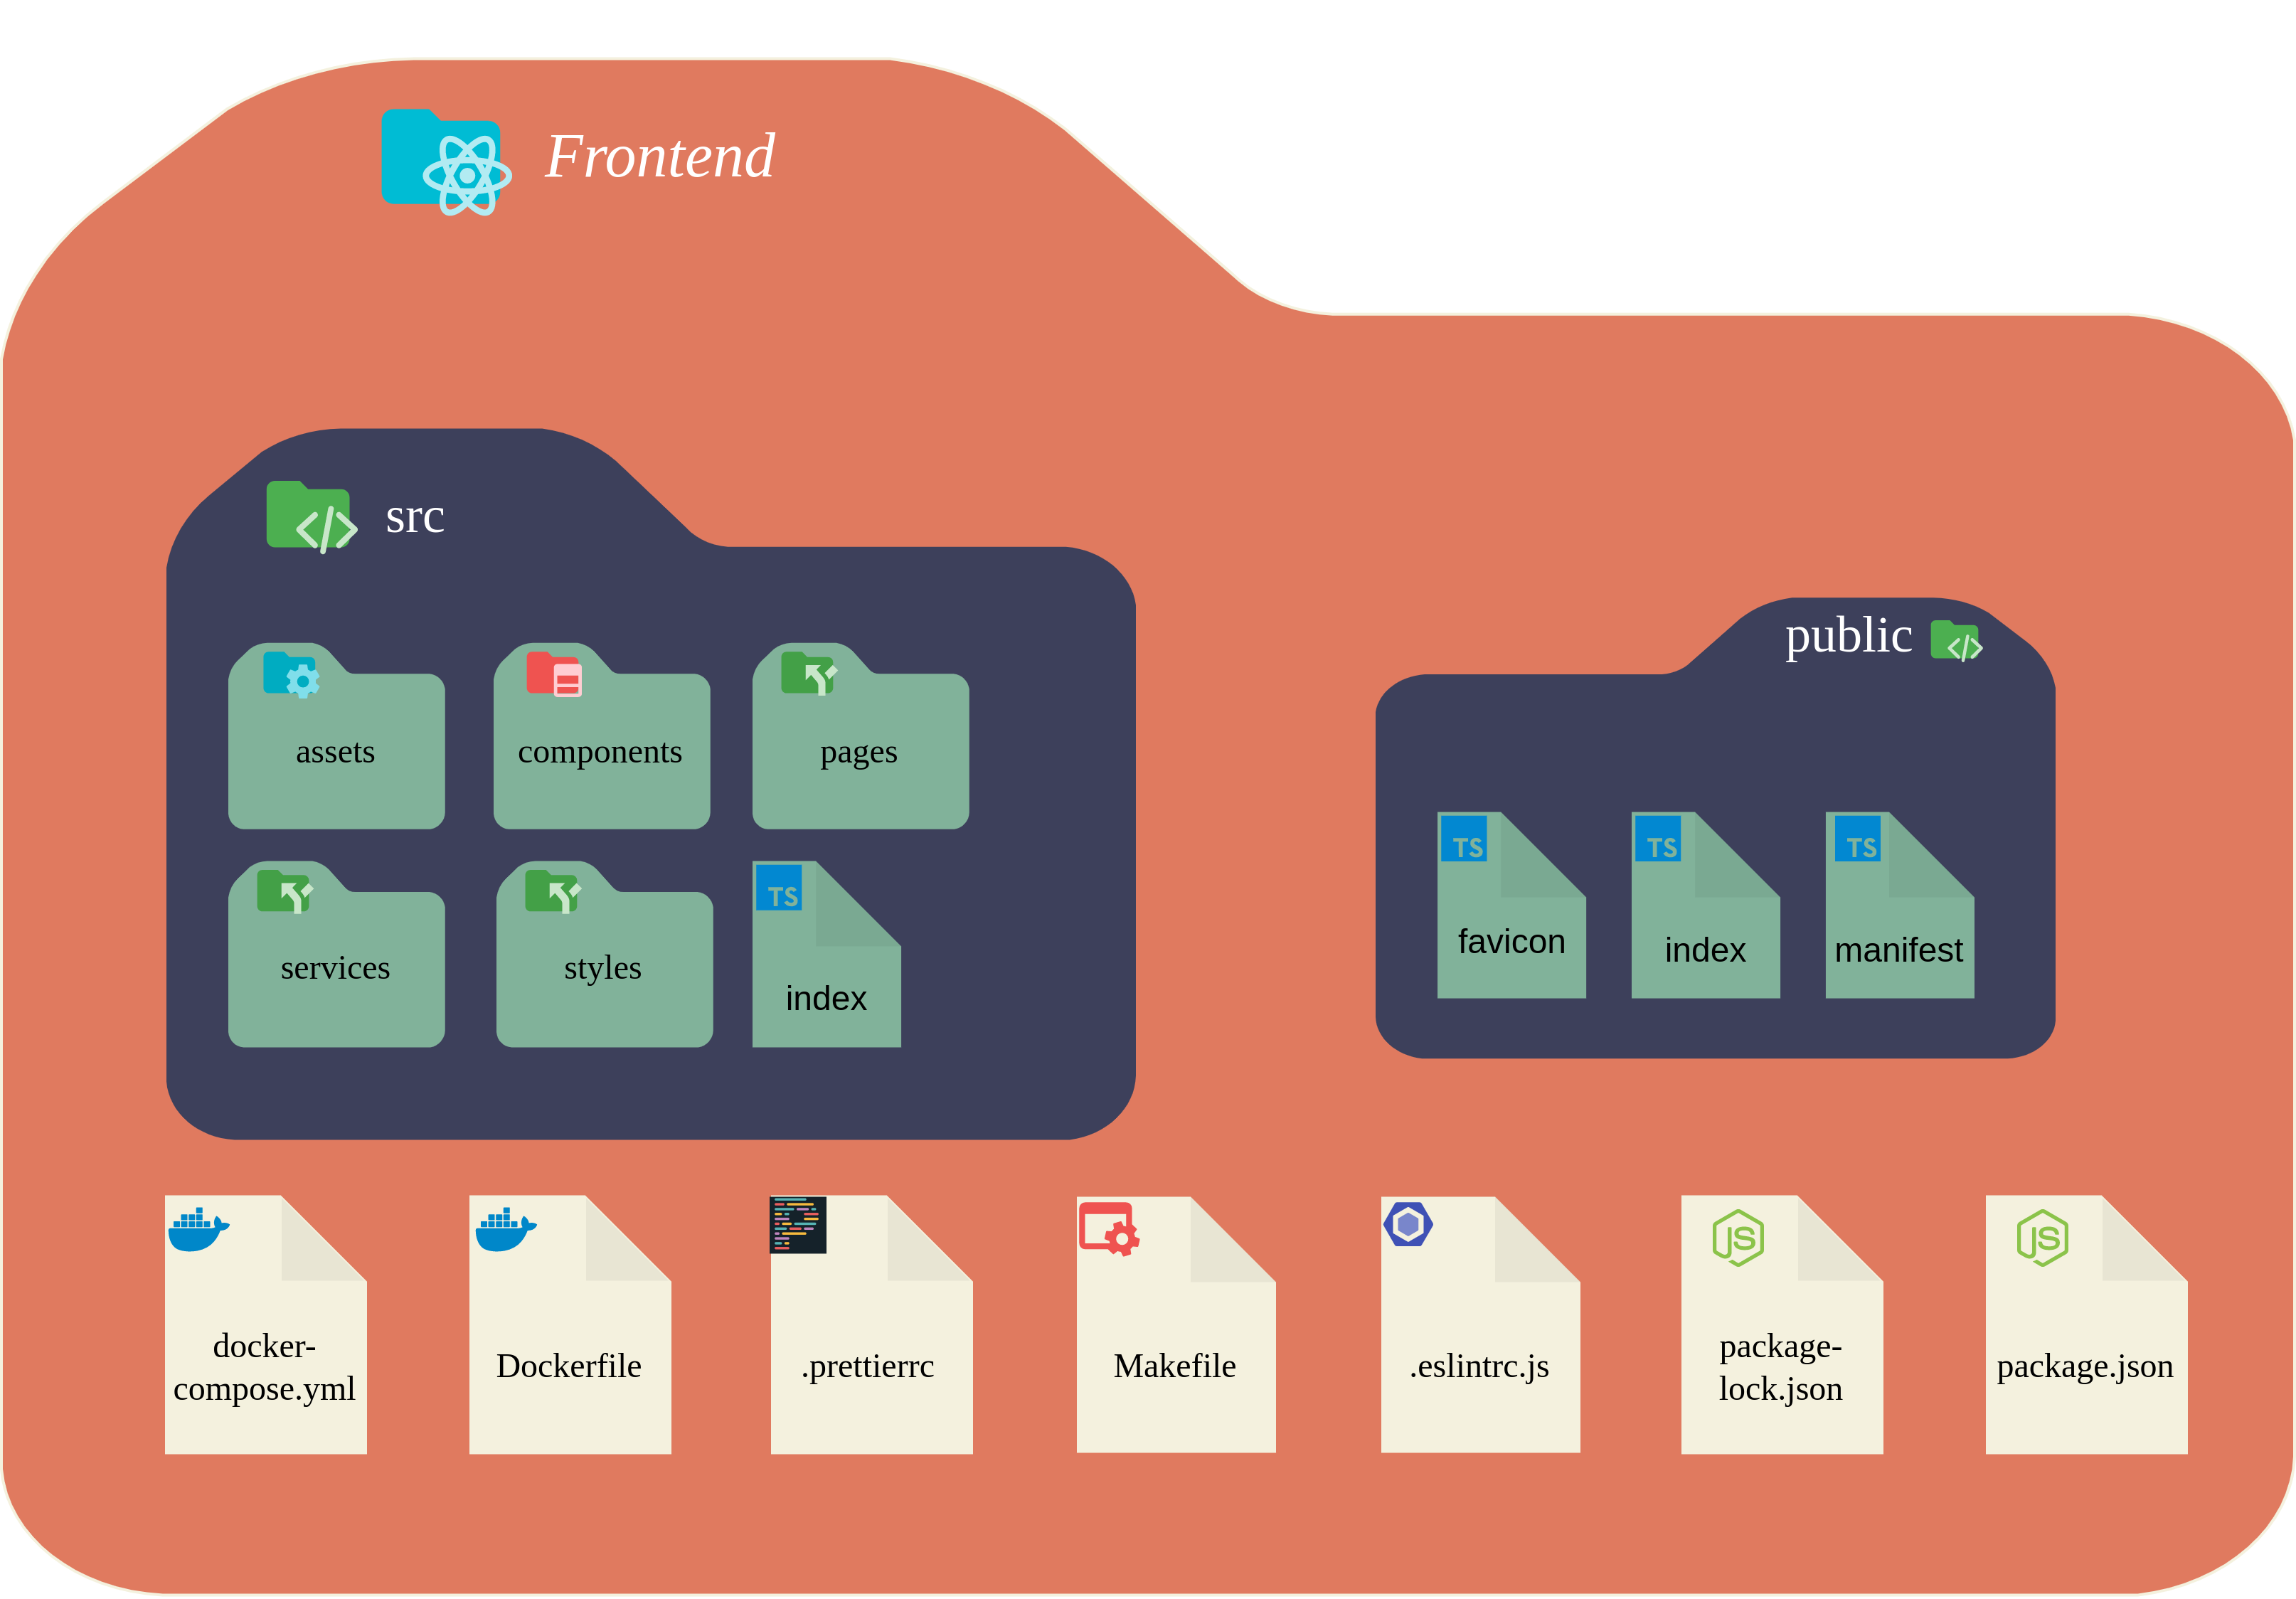
\includegraphics[scale=0.7]{figuras/Proposta/Diagrama_de_Pacotes-Frontend.png}
        \legend{Fonte: Autores, 2022.}
    \end{center}
\end{figure}

\section{Protótipo de Alta Fidelidade}

\label{sec:prototipo_de_alta_fidelidade}

Um protótipo de alta fidelidade deve se aproximar ao máximo dos aspectos visuais e funcionais do produto final, incluindo o conteúdo, fluxo de navegação e interações. São muito utilizados para testes e validação com usuários, ou para apresentar uma ideia. Objetivamente, a ideia do protótipo é saber como a ferramenta funcionará \cite{hf_prototype}.

Com este intuito, foi elaborado um Protótipo de Alta Fidelidade navegável, na plataforma \textit{Figma} \cite{figma}. Como, a quantidade de telas geradas foi demasiadamente grande, foram disponibilizadas apenas algumas das muitas telas desenvolvidas, para evidenciar, ainda que em suma, qual o perfil do produto. Entretanto, para visualizar todas as telas e poder navegar e interagir, optou-se por disponibilizar o enlace para ser acessado \textit{on-line}: \citeauthoronline{prototipo_alta_fidelidade} (\citeyear{prototipo_alta_fidelidade}).

Estão elencadas a seguir as principais telas desenhadas para o \textit{iFlow}:

\begin{itemize}
    \item A Figura \ref{fig:cards_etapas_prototipo} trata da página onde estão elencadas todas as etapas necessárias para o desenvolvimento da Engenharia de Requisitos, proposto para a ferramenta \textit{iFlow};
    \begin{figure}[]
      \begin{center}
          \caption{{Tela das Etapas da Engenharia de Requisitos do Protótipo}}
          \label{fig:cards_etapas_prototipo}
          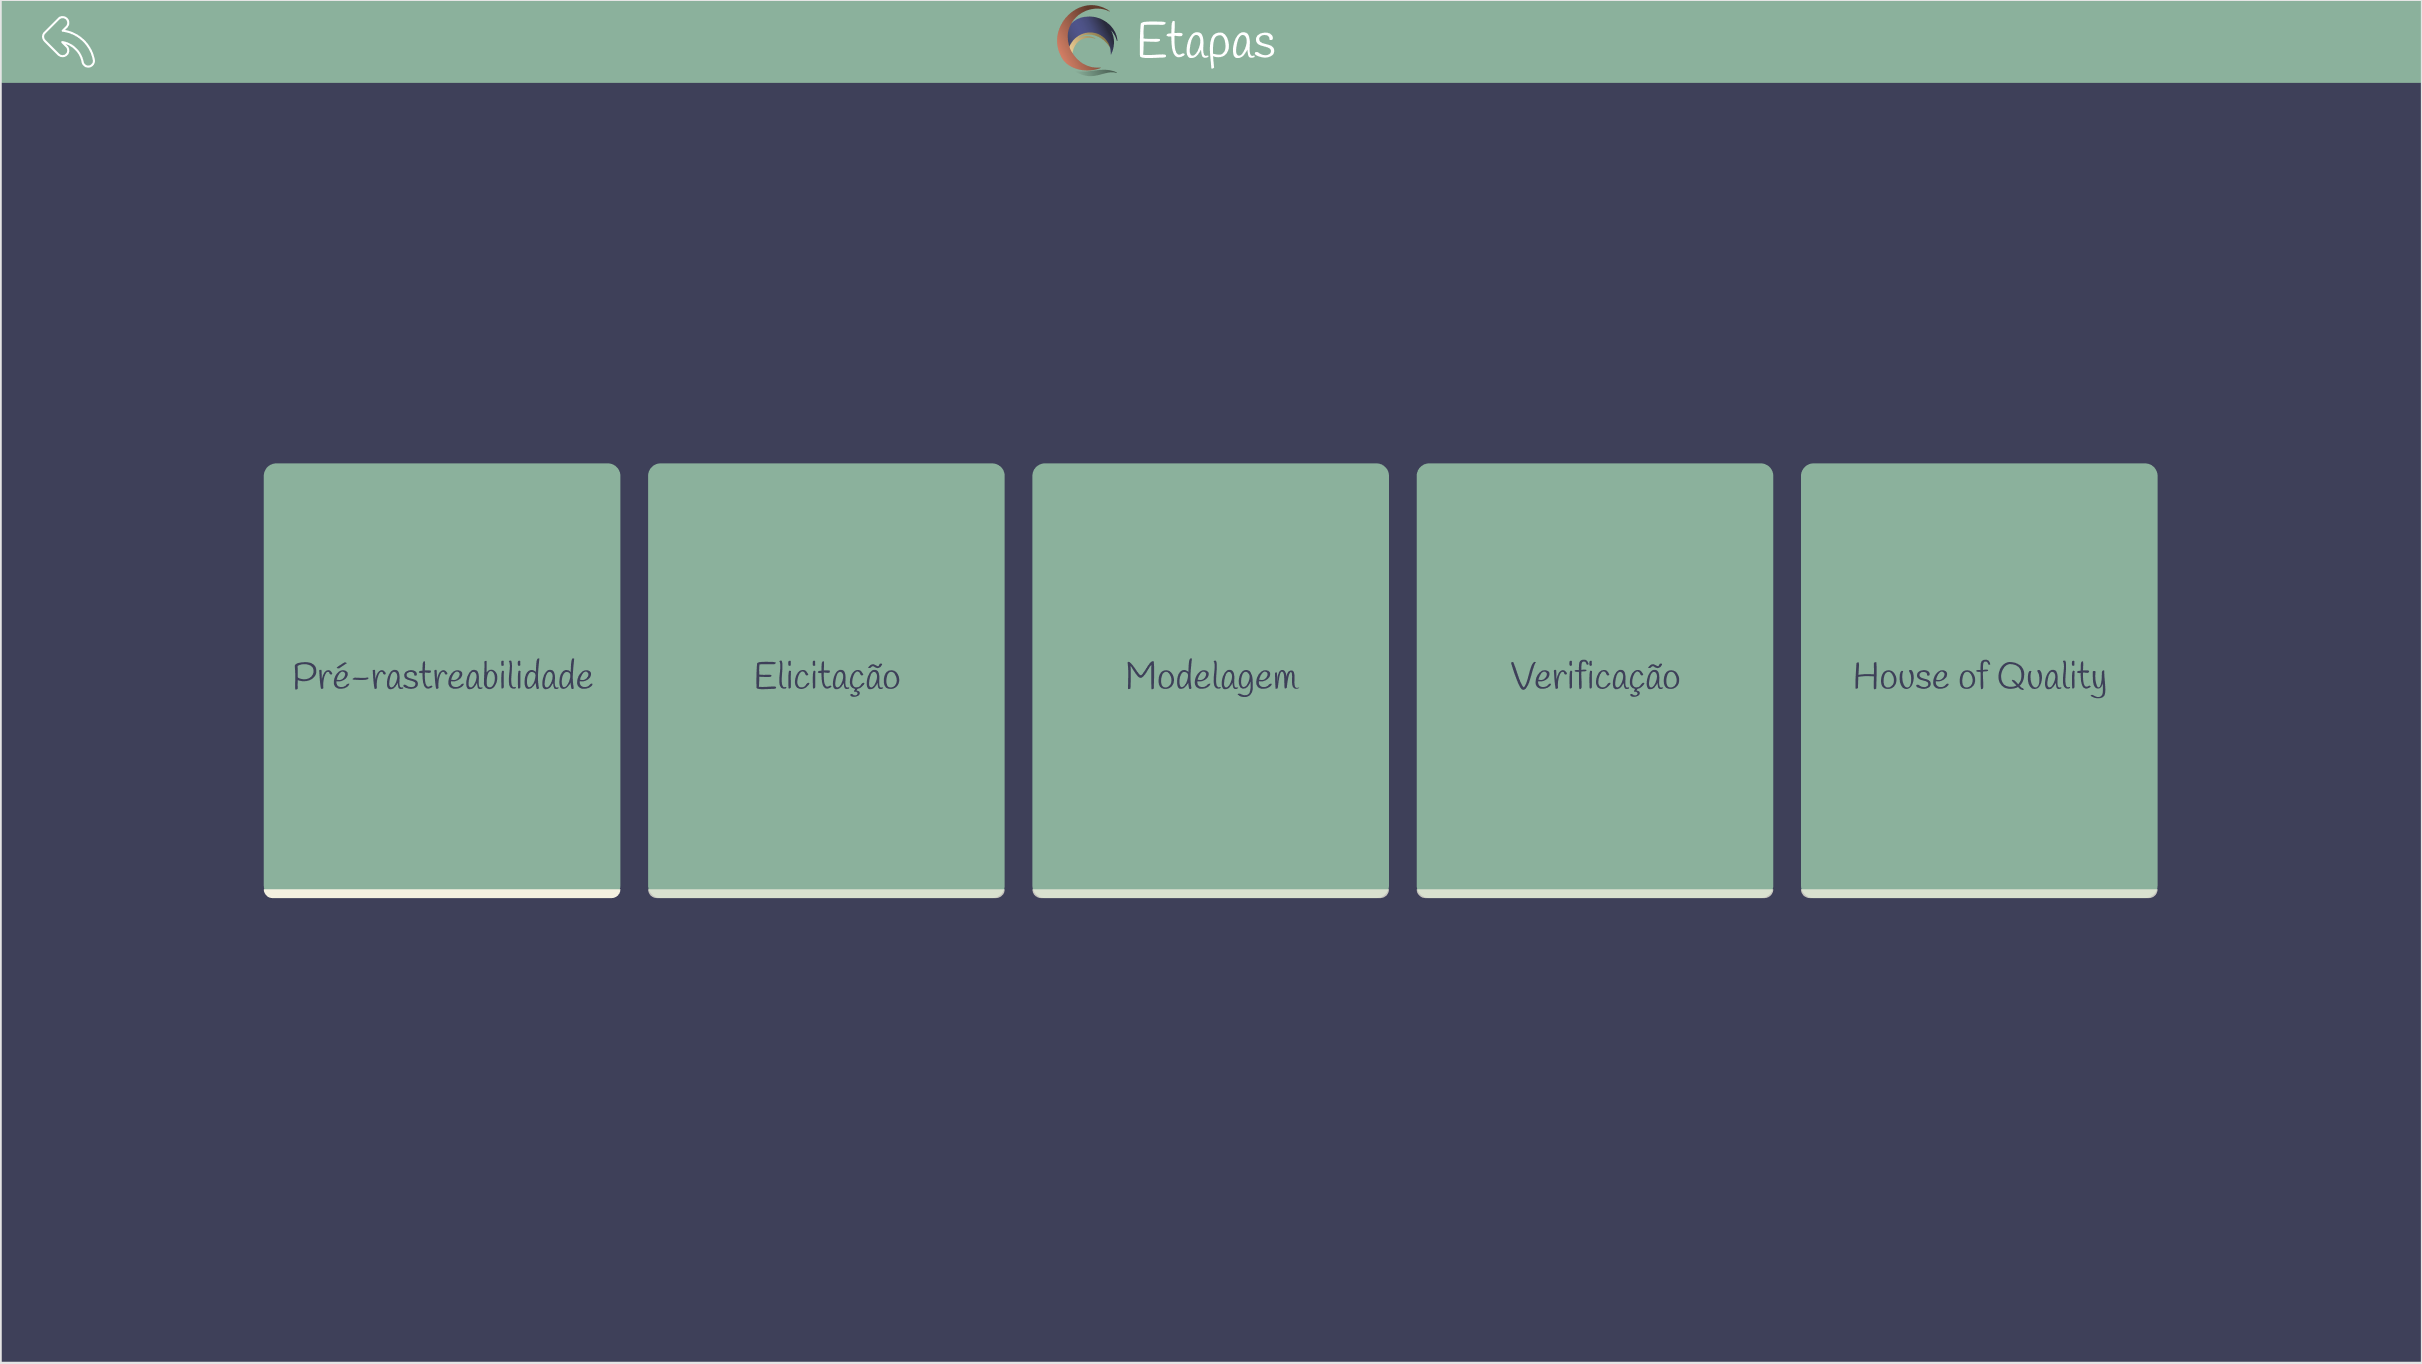
\includegraphics[scale=0.36]{figuras/Prototipo/etapas.png}
        \legend{Fonte: Autores, 2022.}
    \end{center}
    \end{figure}
    \item A Figura \ref{fig:completed_artifacts} trata da tela onde são listados os artefatos que já foram concluídos, que, neste caso, se trata dos gerados na elicitação do projeto em questão;
    \begin{figure}[]
      \begin{center}
          \caption{{Tela dos Artefatos Elaborados}}
          \label{fig:completed_artifacts}
          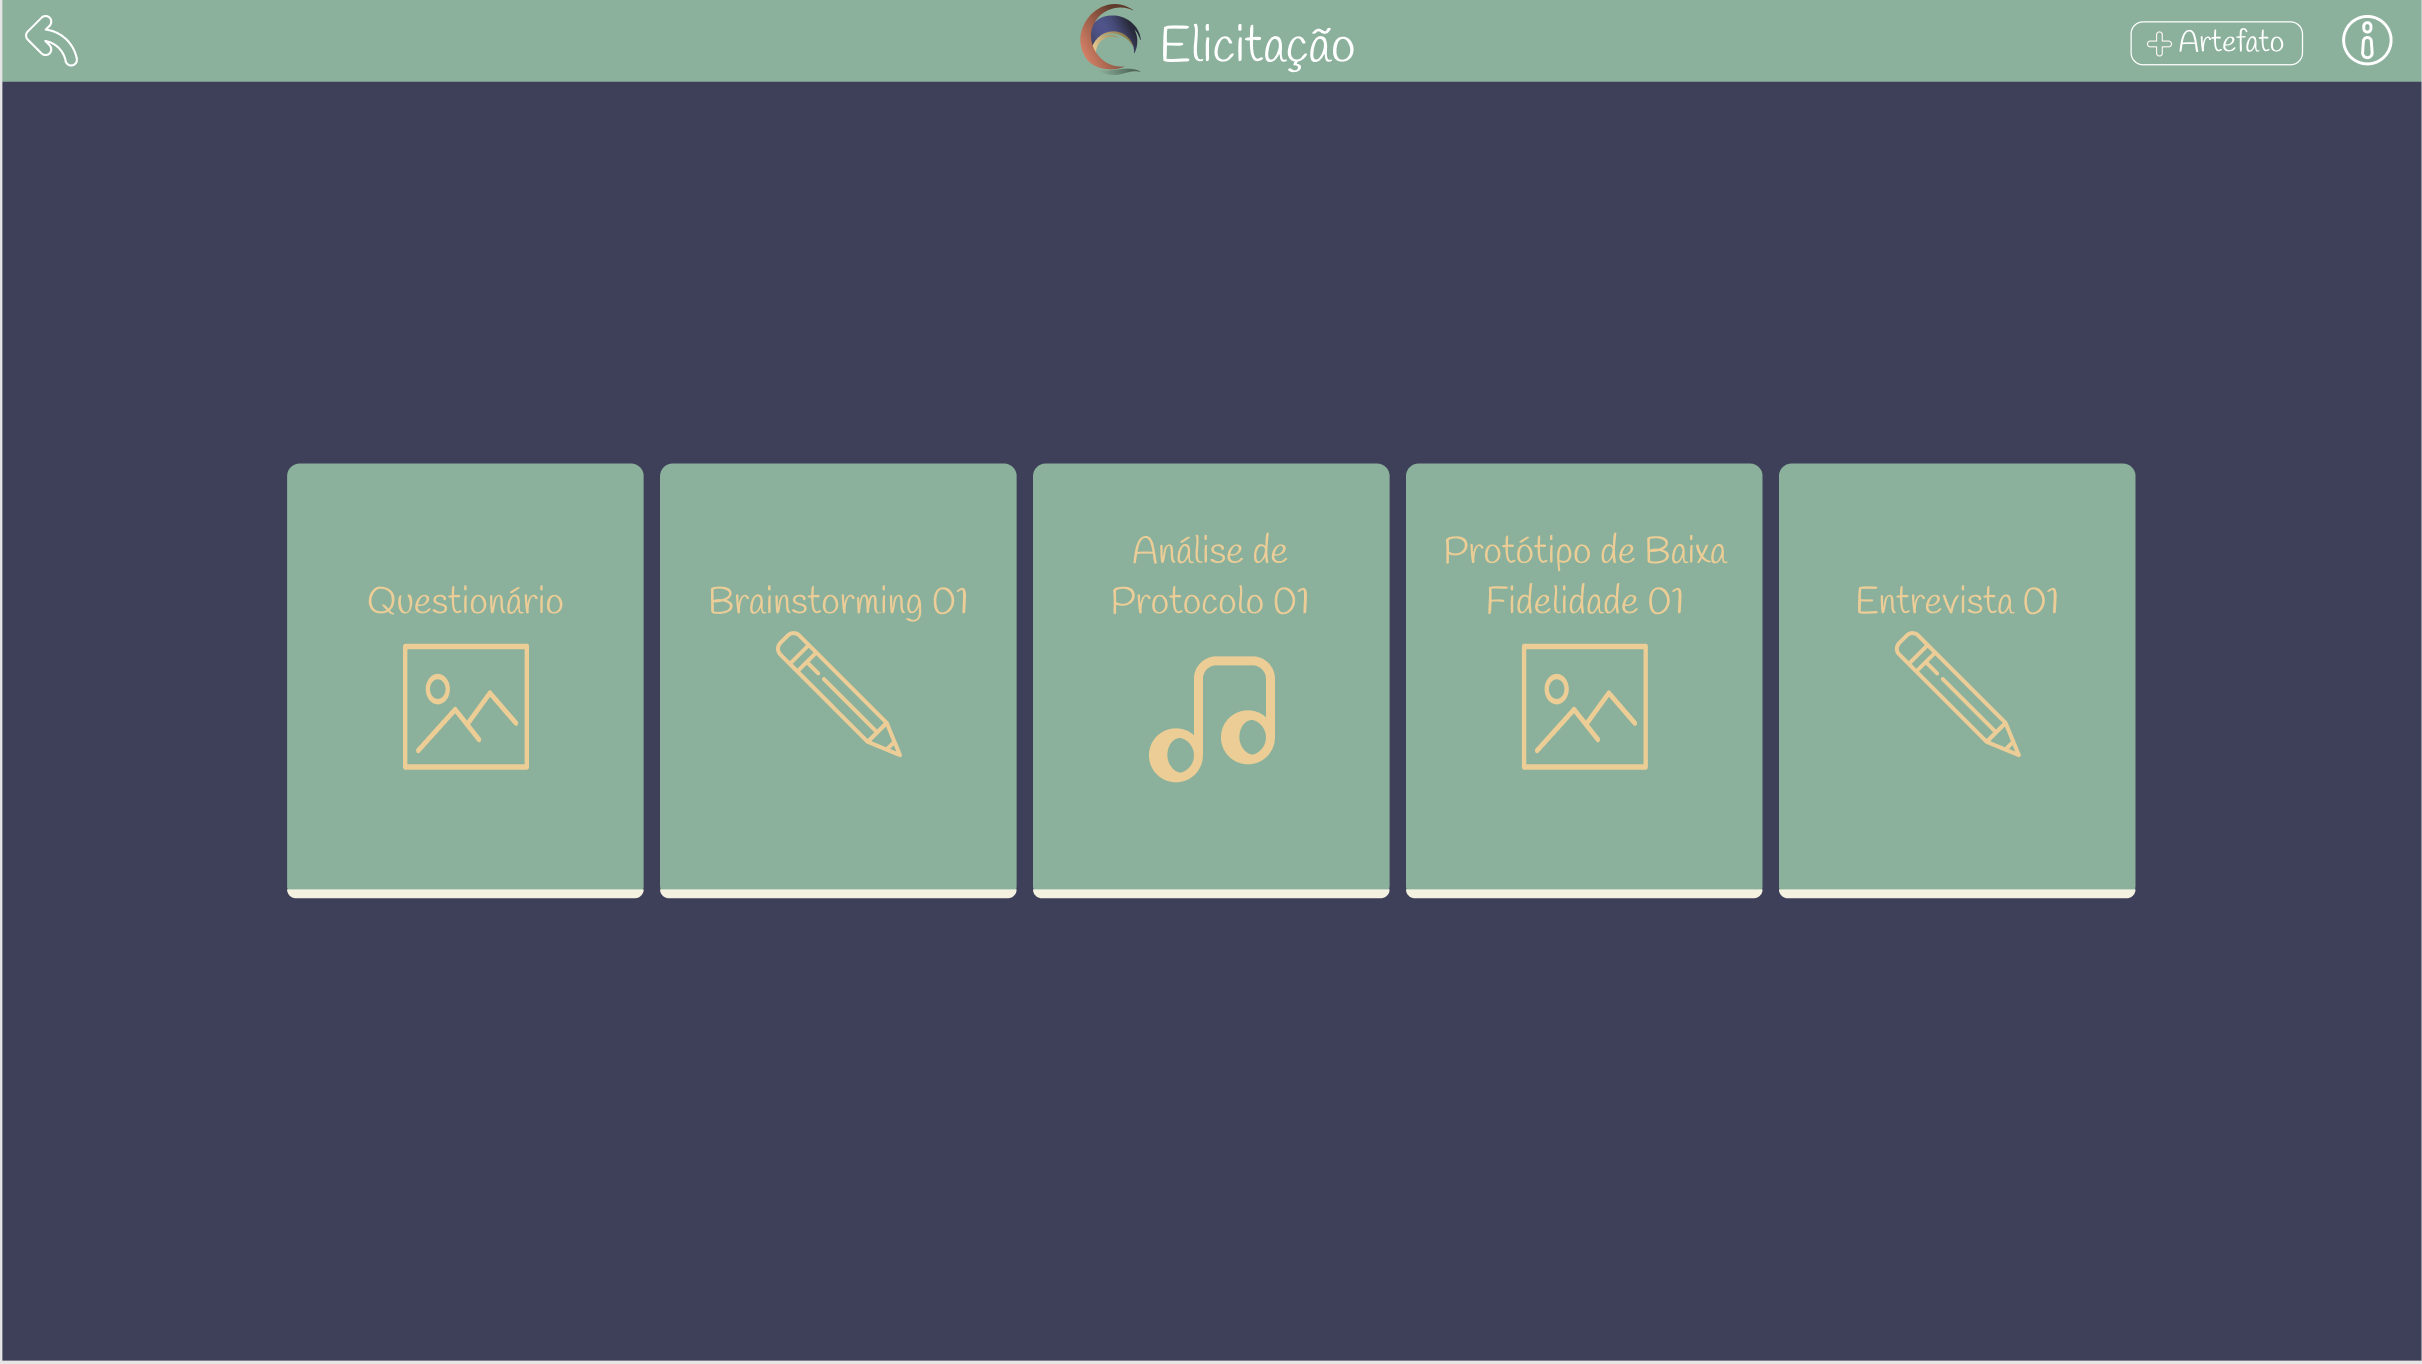
\includegraphics[scale=0.36]{figuras/Prototipo/completed-artifacts.png}
        \legend{Fonte: Autores, 2022.}
    \end{center}
    \end{figure}
    \item A Figura \ref{fig:backlog_prototipo} representa as telas de criação do \textit{Backlog} do Produto e da \textit{House of Quality}, que as etapas de suma importância dentro deste processo, e
    \begin{figure}[]
      \begin{center}
          \caption{{Telas de Criação do \textit{Backlog} do Produto e da \textit{House of Quality}, respectivamente}}
          \label{fig:backlog_prototipo}
          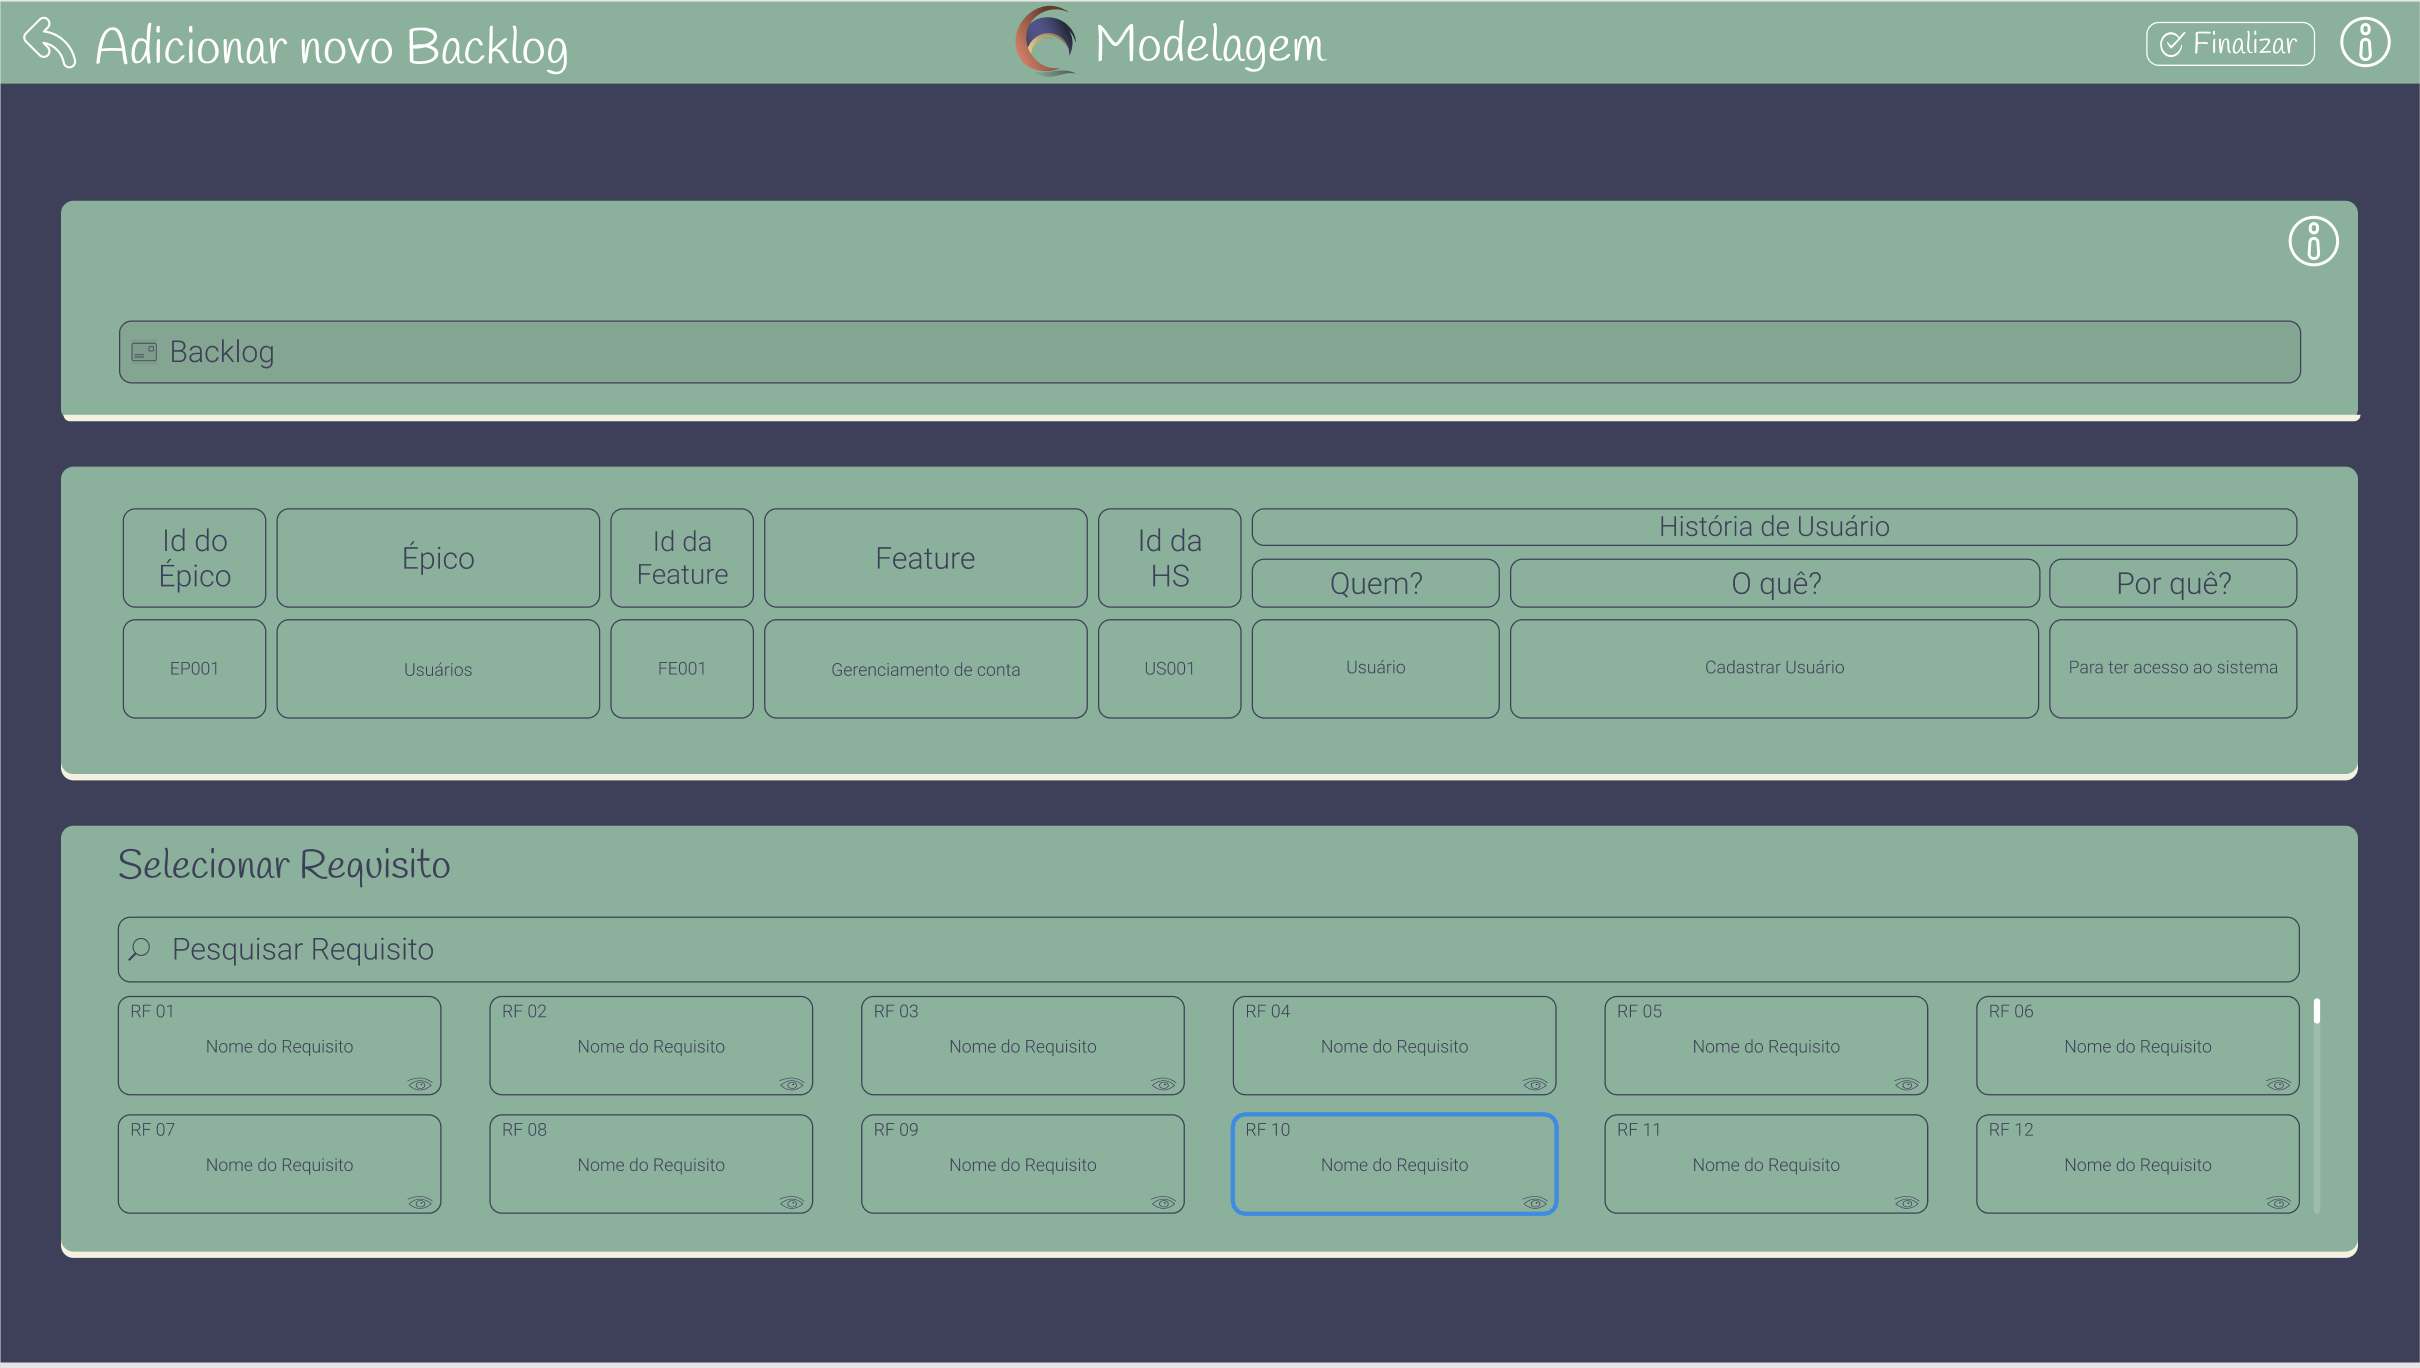
\includegraphics[scale=0.36]{figuras/Prototipo/backlog.png}
          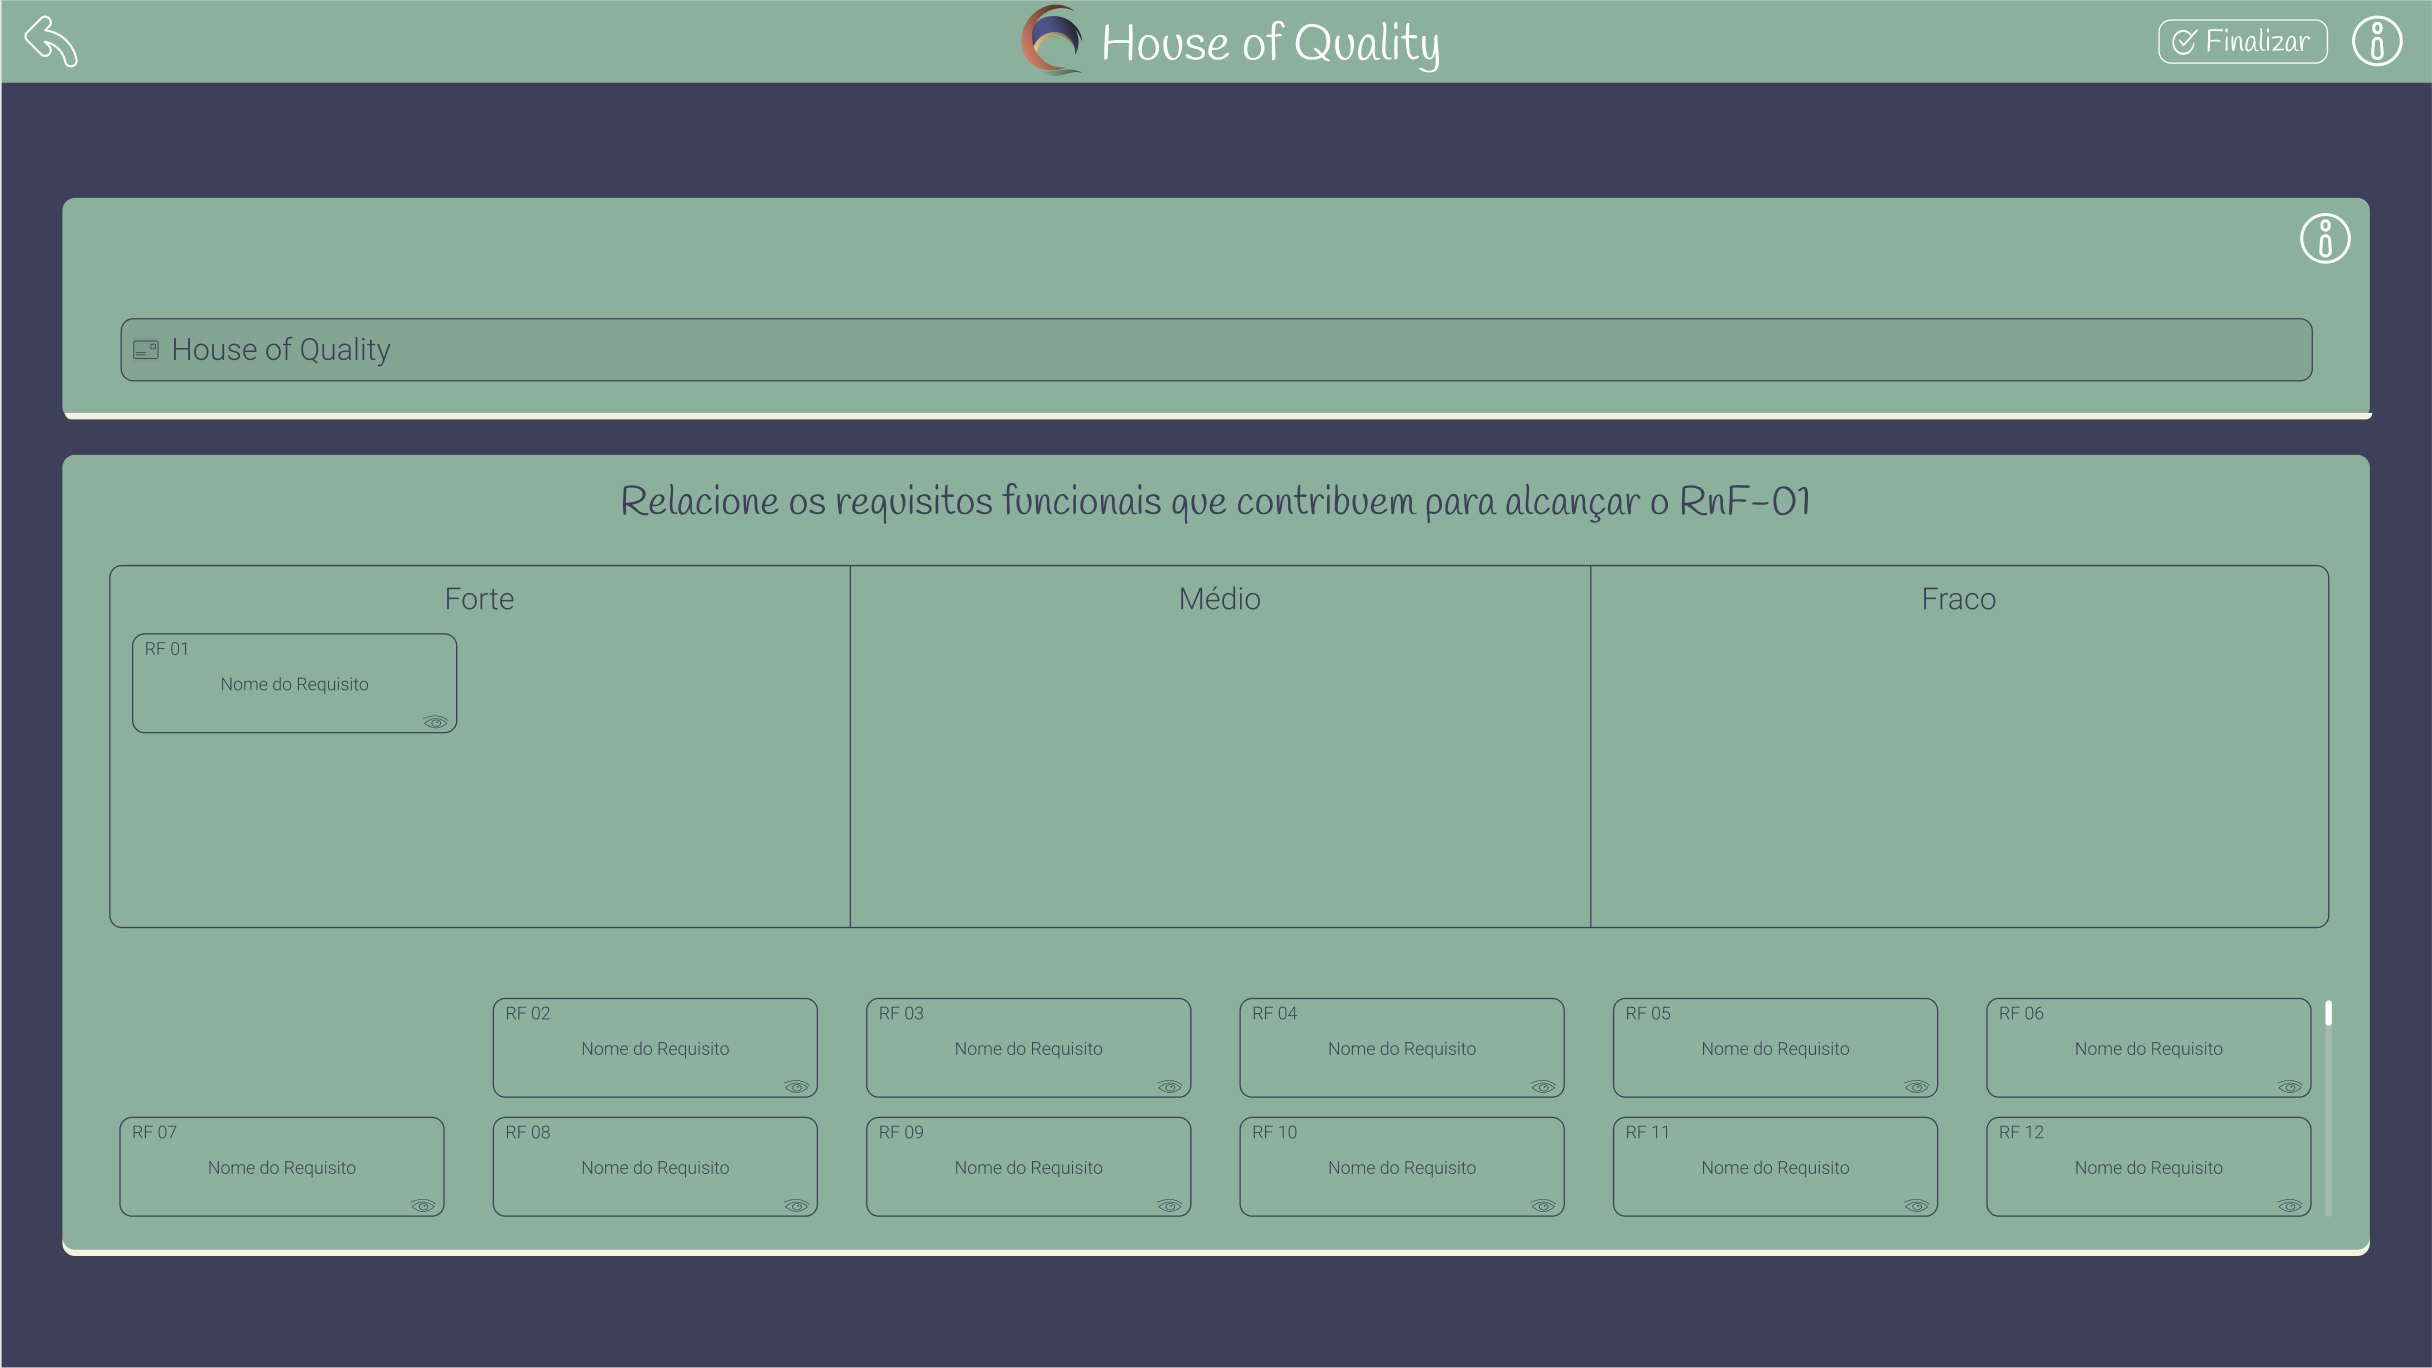
\includegraphics[scale=0.36]{figuras/Prototipo/house-of-quality.png}
        \legend{Fonte: Autores, 2022.}
    \end{center}
    \end{figure}
    \item Por fim, tem-se a Figura \ref{fig:mvp} com a tela de renderização do Produto Mínimo Viável gerado, em sua versão preliminar.
    \begin{figure}[]
      \begin{center}
          \caption{{Tela com o Produto Mínimo Viável da Aplicação em sua Versão Preliminar}}
          \label{fig:mvp}
          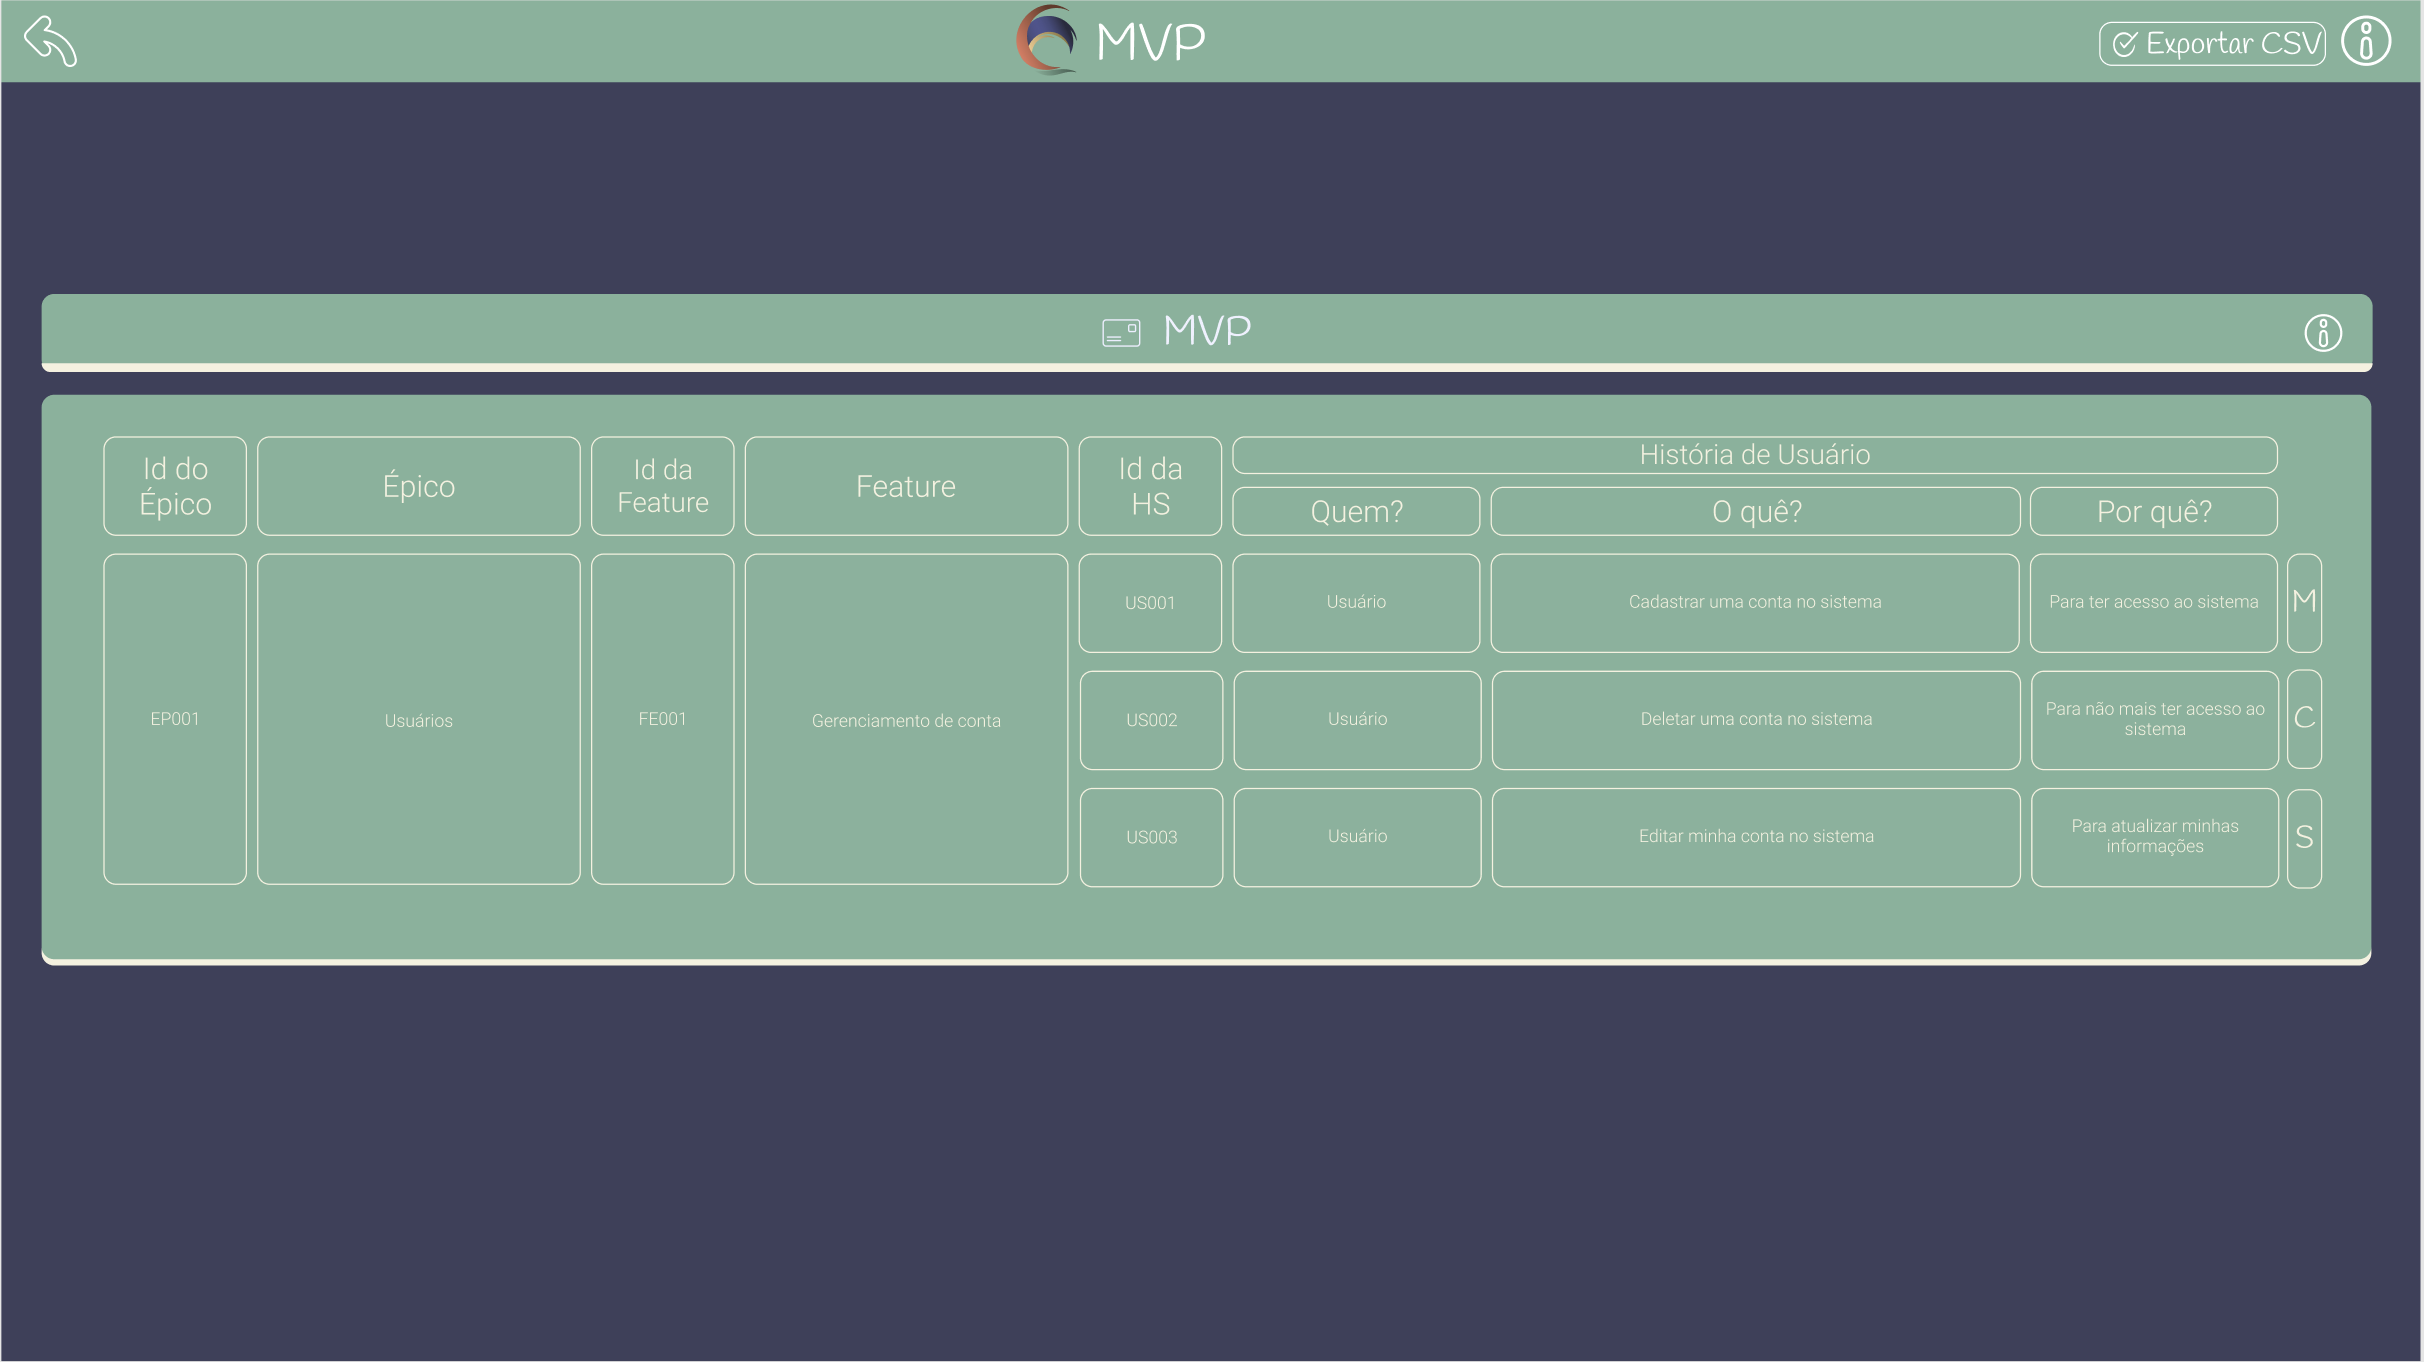
\includegraphics[scale=0.36]{figuras/Prototipo/mvp.png}
        \legend{Fonte: Autores, 2022.}
    \end{center}
    \end{figure}
\end{itemize}

\section{\textit{Backlog} do Produto}

\label{sec:backlog_do_produto}

Com o intuito de guiar o processo de desenvolvimento da ferramenta \textit{iFlow}, foi elaborado um \textit{backlog} com os requisitos necessários para compor a aplicação. As definições, e correspondente tabela, foram colocadas no Apêndice \ref{ap:backlog}.

\section{Versão Final — \textit{iFlow}}
\label{sec:versao_final_iFlow}

\subsection{Telas desenvolvidas}

A versão final das telas não se difere muito em relação ao protótipo de alta fidelidade (Seção \ref{sec:prototipo_de_alta_fidelidade}). Todavia, algumas telas tiveram que ser simplificadas, para que se pudesse desenvolver todas as telas indispensáveis ao projeto, ou foram melhoradas em algum aspecto visual que não ficou tão satisfatório no protótipo de alta fidelidade.

Como foram desenvolvidas muitas telas, a seguir, foram elencadas as telas mais relevantes da ferramenta, correspondentes às apresentadas no protótipo de alta fidelidade (Seção \ref{sec:prototipo_de_alta_fidelidade}), sendo elas:

\begin{itemize}
    \item A Figura \ref{fig:etapas_implementado} retrata a tela das Etapas da Engenharia de Requisitos em sua versão final, mostrando semelhança em relação ao protótipo desenvolvido;
    \begin{figure}[]
      \begin{center}
          \caption{{Tela das Etapas em sua Versão Final}}
          \label{fig:etapas_implementado}
          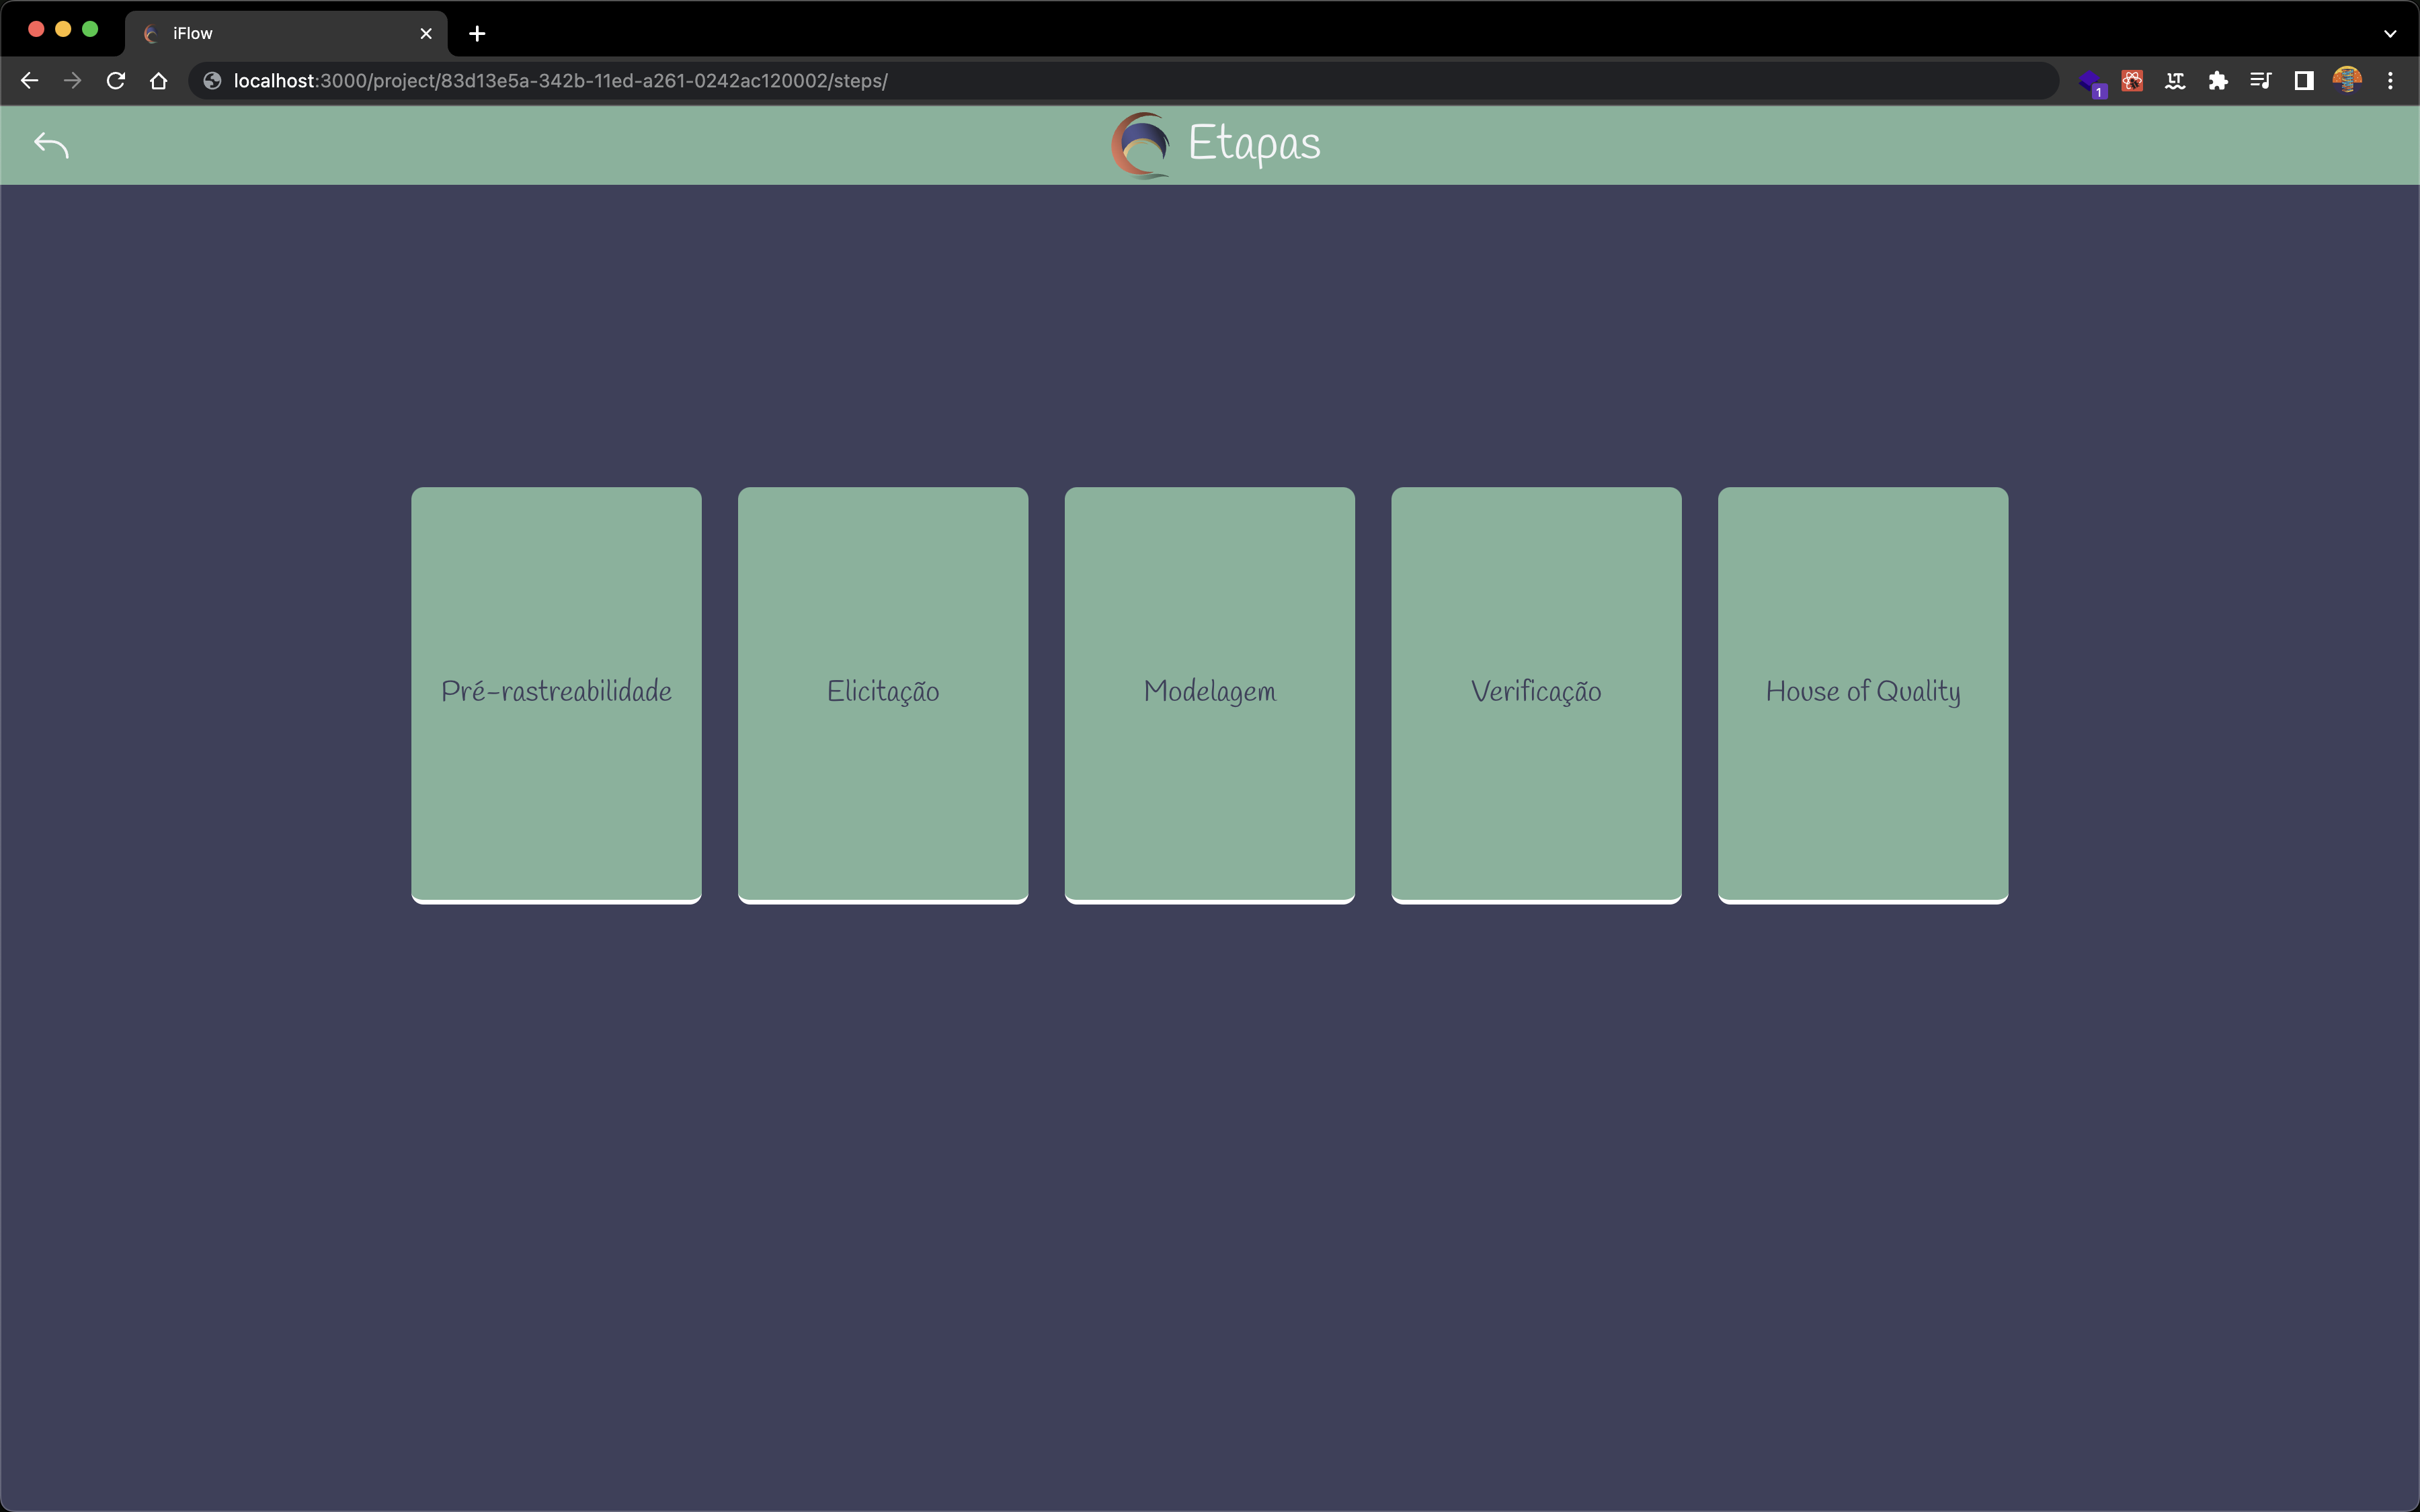
\includegraphics[scale=0.24]{figuras/TelasDesenvolvidas/etapas-implementado.png}
        \legend{Fonte: Autores, 2022.}
    \end{center}
    \end{figure}
    
    \item A Figura \ref{fig:artefatos_completos_implementado} exibe os artefatos finalizados na etapa de elicitação, mostrando semelhança com o protótipo desenvolvido;
    \begin{figure}[]
      \begin{center}
          \caption{{Tela dos Artefatos Elaborados em sua Versão Final}}
          \label{fig:artefatos_completos_implementado}
          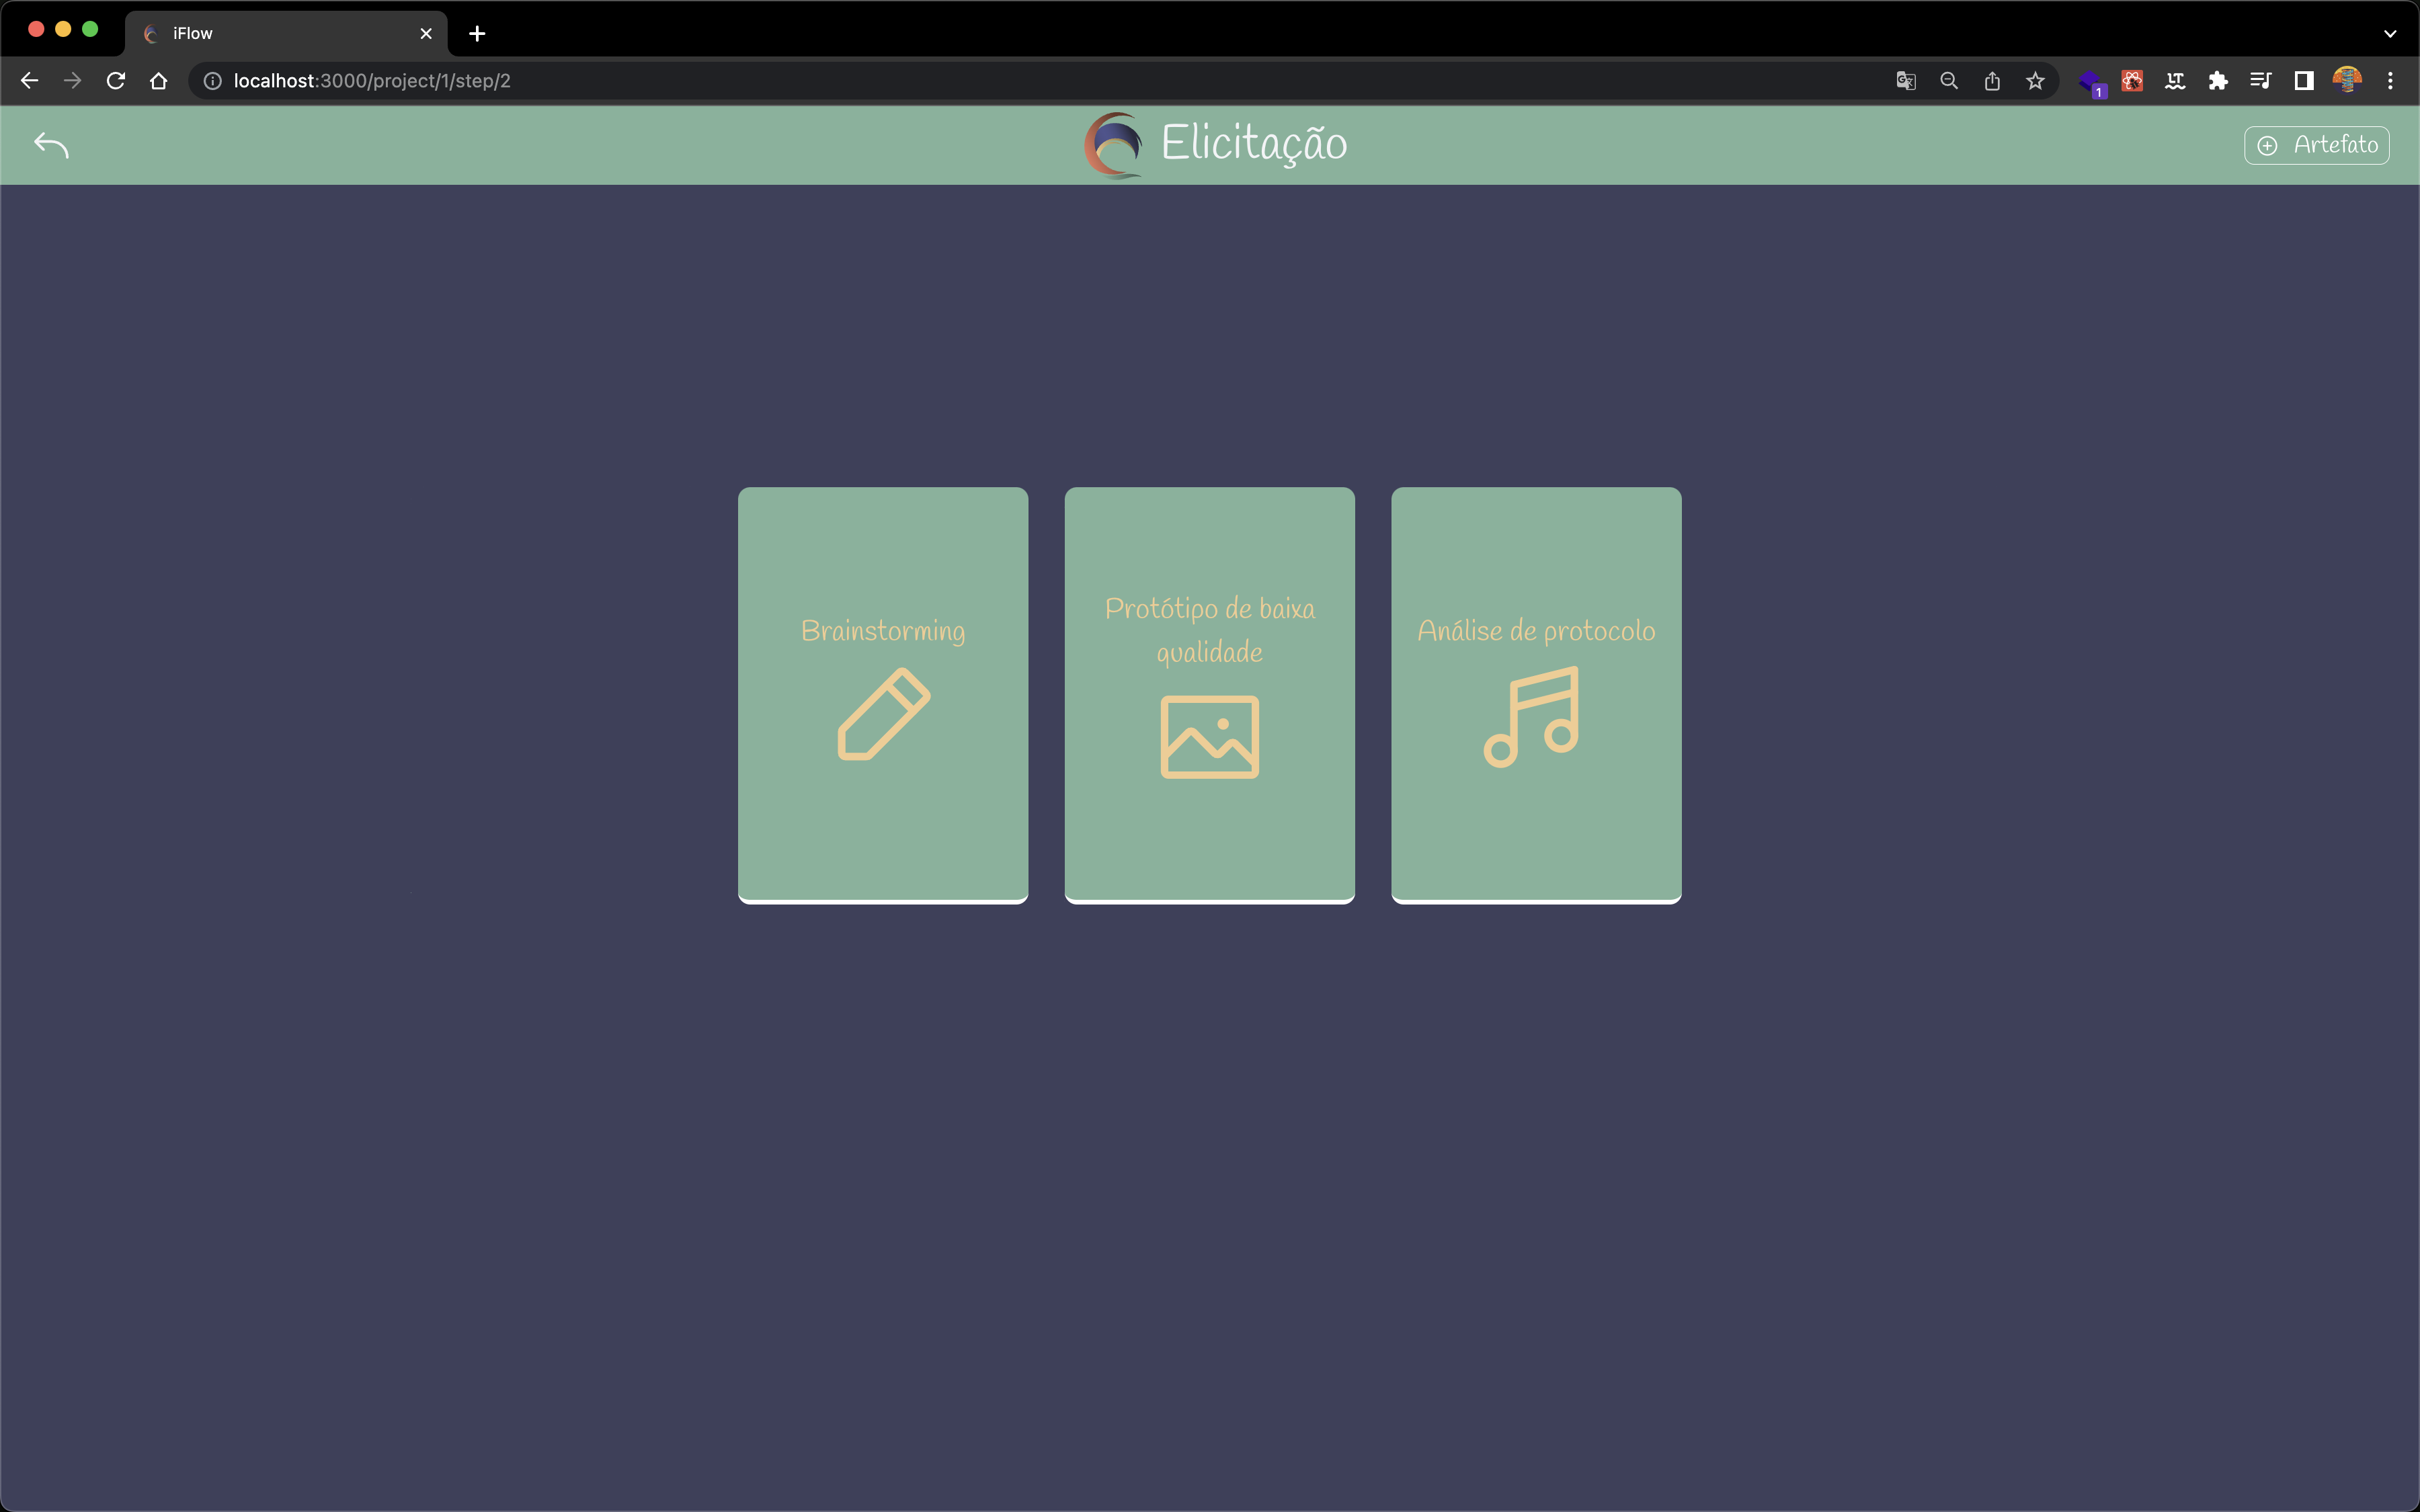
\includegraphics[scale=0.24]{figuras/TelasDesenvolvidas/completed-artifacts-implementado.png}
        \legend{Fonte: Autores, 2022.}
    \end{center}
    \end{figure}
    
    \item A Figura \ref{fig:novo_artefato} revela a criação de um novo artefato, nesse caso, um novo Questionário. Pode-se observar que essa tela possui algumas divergências em relação ao protótipo, onde os requisitos são listados abaixo do conteúdo do artefato, possuindo uma visualização menos adequada. Tendo isso em vista, a melhora de visualização e interface do \textit{iFlow} ficariam como trabalhos futuros;
    \begin{figure}[]
      \begin{center}
          \caption{{Tela de Criação de um Novo Artefato}}
          \label{fig:novo_artefato}
          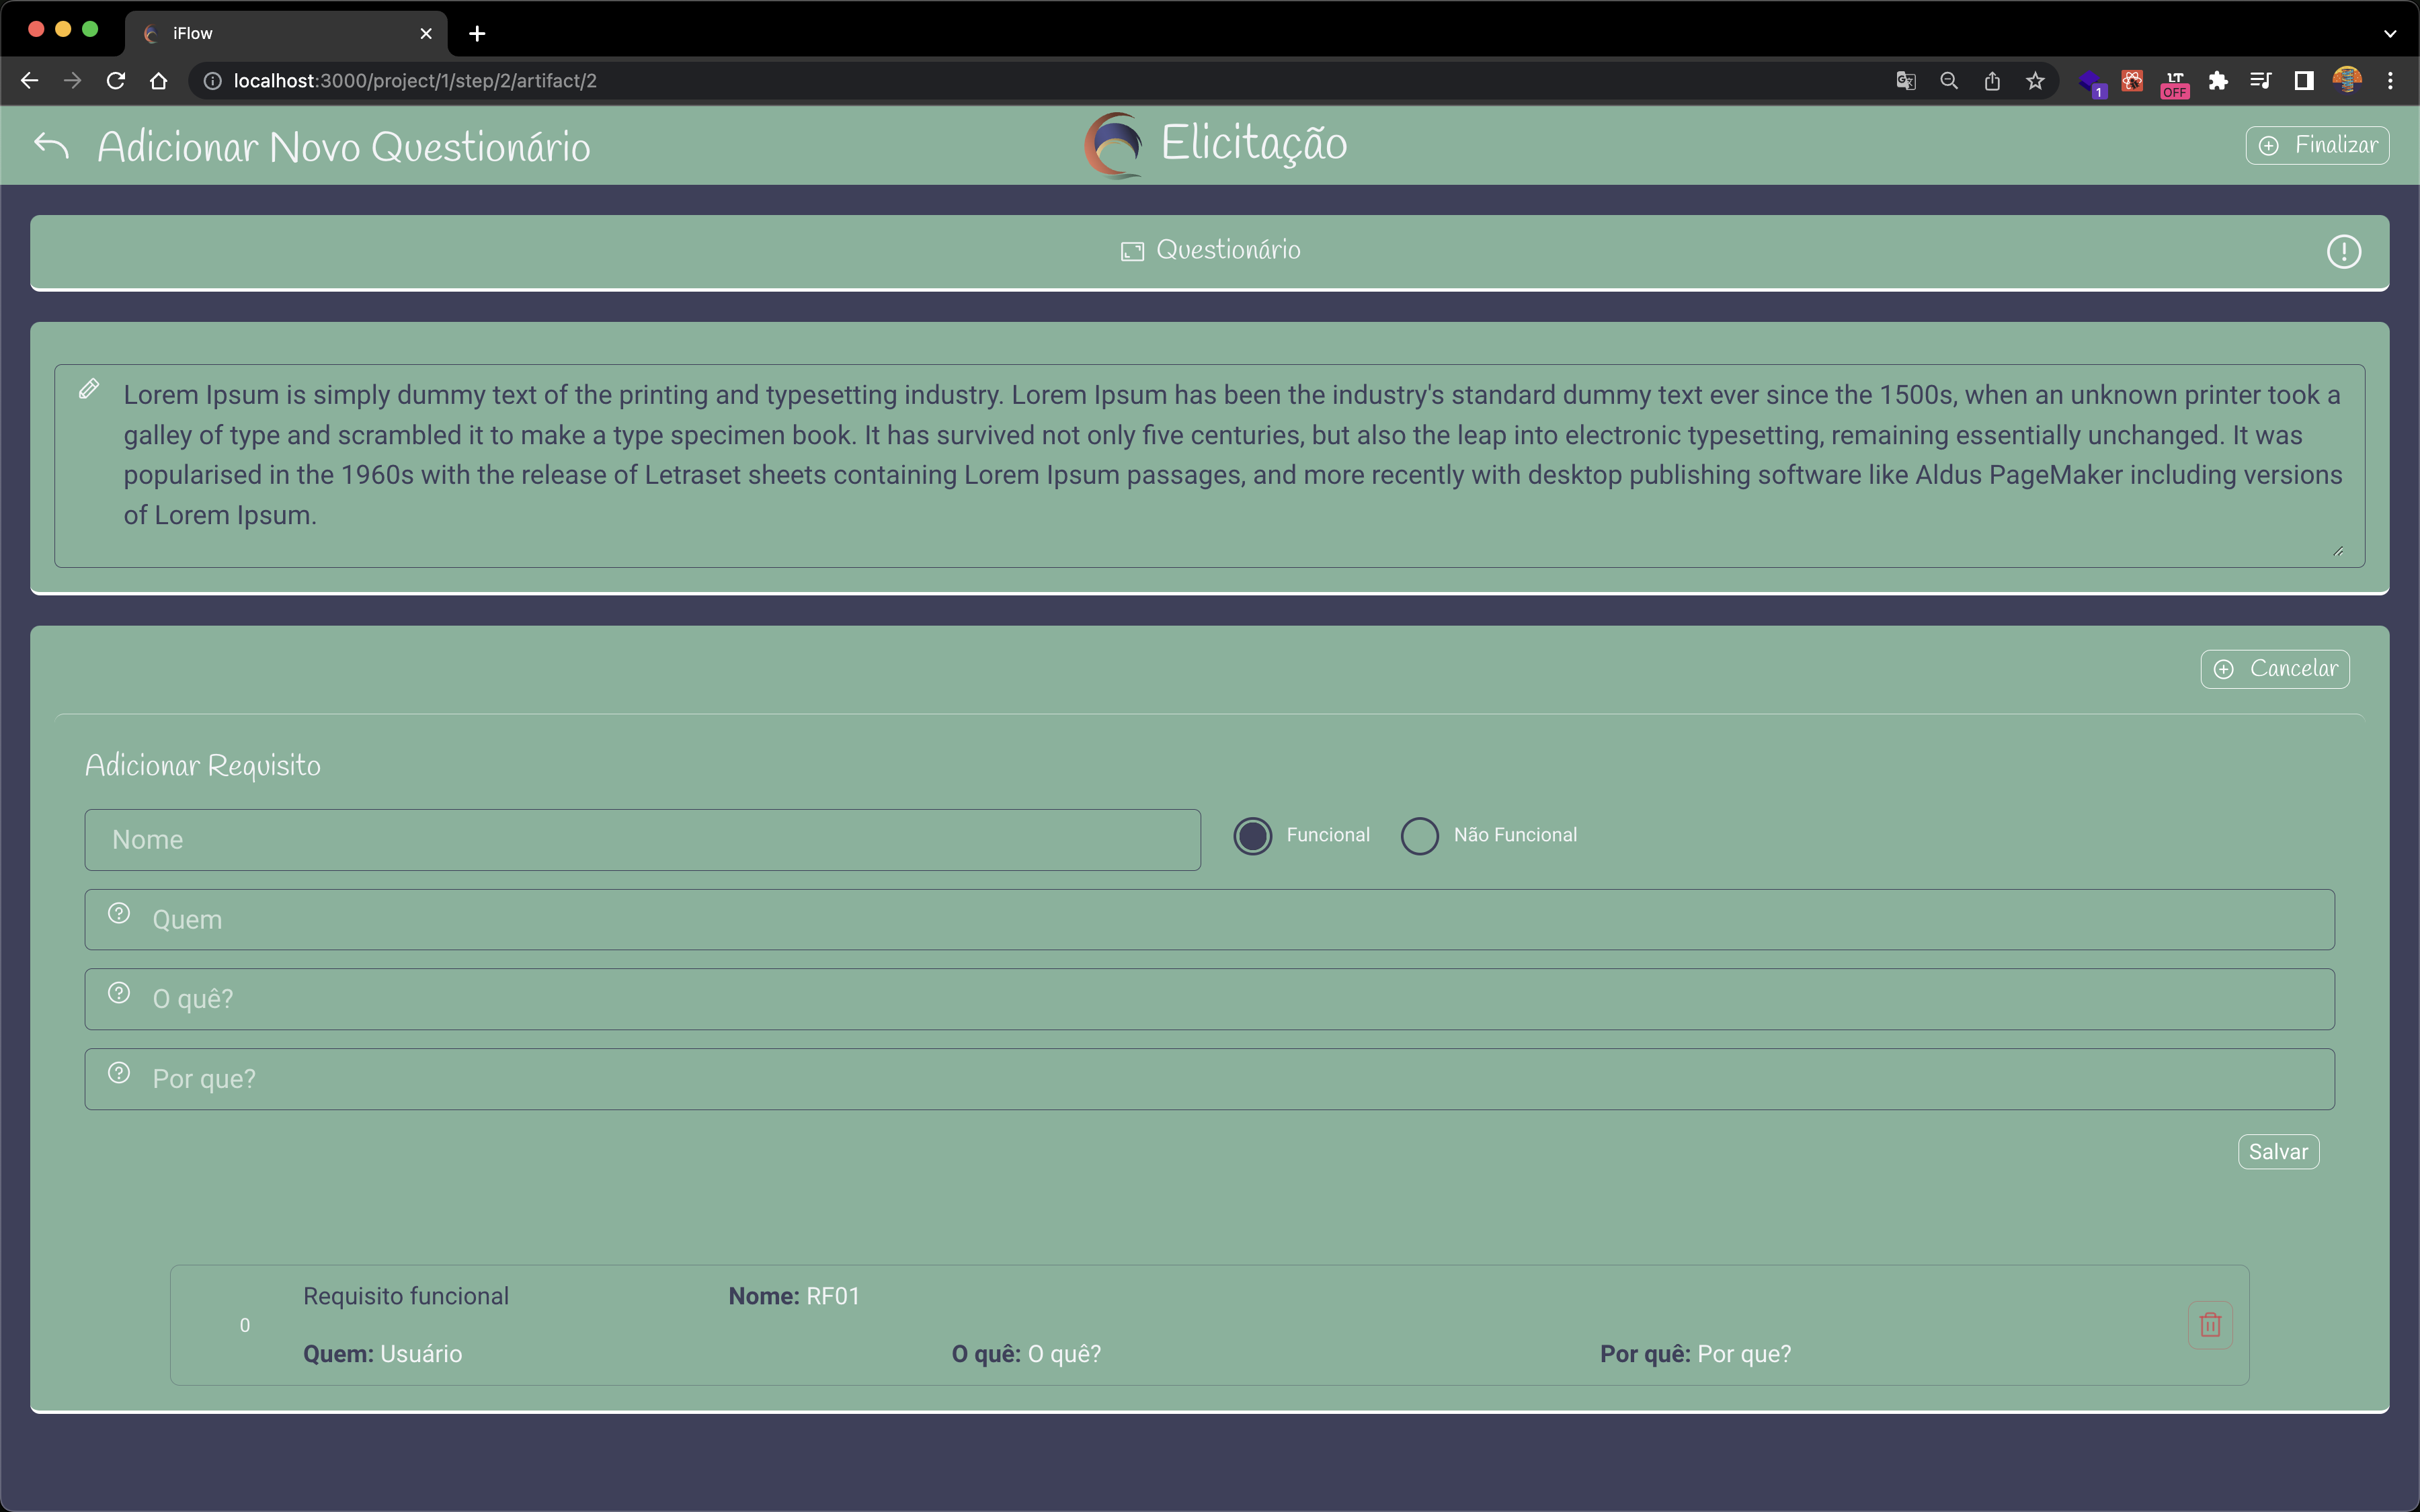
\includegraphics[scale=0.22]{figuras/TelasDesenvolvidas/new-artifact.png}
        \legend{Fonte: Autores, 2022.}
    \end{center}
    \end{figure}

    \item A Figura \ref{fig:backlog_implementado} representa a criação do \textit{Backlog} do Produto em sua versão final. É uma tela de suma importância no contexto de Engenharia de Requisitos, sendo bem semelhante à desenvolvida no protótipo, além de ter a funcionalidade de arrastar o requisito funcional para a tabela do \textit{Backlog}, e
    \begin{figure}[]
      \begin{center}
          \caption{{Tela de Criação do \textit{Backlog} do Produto em sua Versão Final}}
          \label{fig:backlog_implementado}
          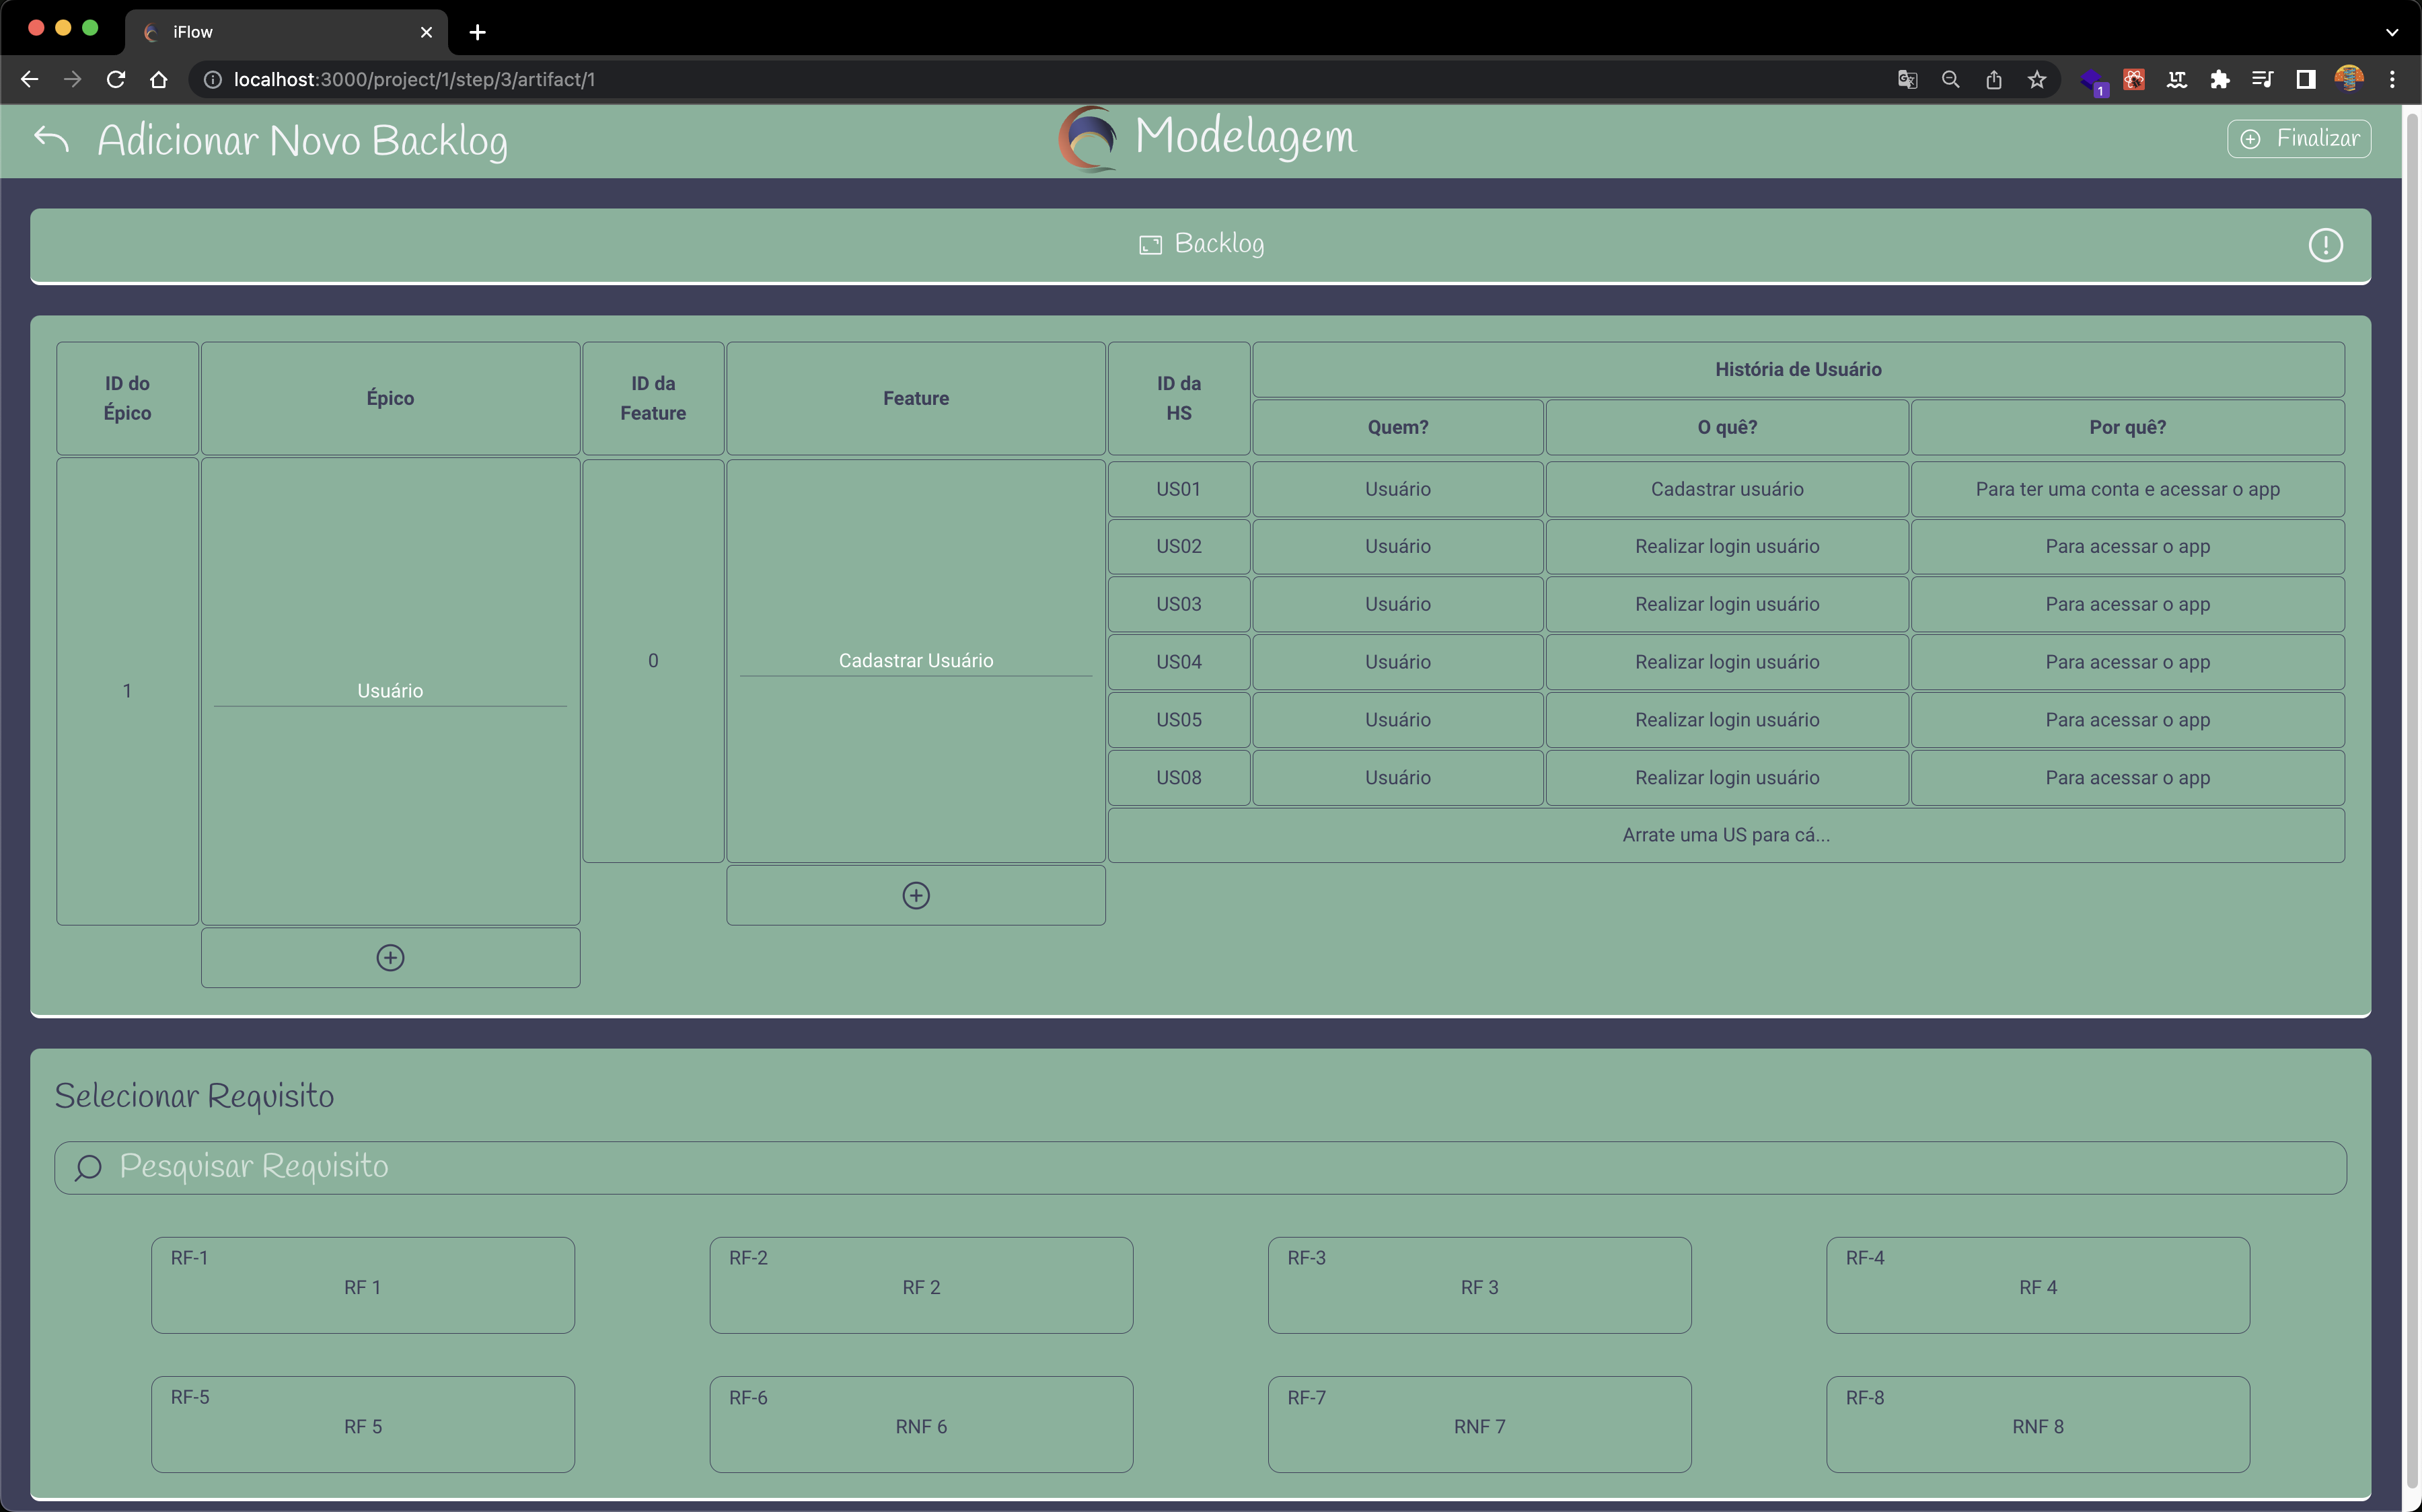
\includegraphics[scale=0.22]{figuras/TelasDesenvolvidas/backlog-implementado.png}
        \legend{Fonte: Autores, 2022.}
    \end{center}
    \end{figure}

    \item Por fim, tem-se a Figura \ref{fig:house_of_quality_implementado}, a qual representa a tela de criação da \textit{House of Quality} em sua versão final. Pode-se reparar que esta tela se assemelha bastante com a desenvolvida no protótipo, possuindo a funcionalidade de arrastar os requisitos funcionais para as respectivas relações com os requisitos não funcionais advindos da etapa do NFR, definindo essa relação como fraca, média ou forte.
    \begin{figure}[]
      \begin{center}
          \caption{{Tela de criação da \textit{House of Quality} em sua Versão Final}}
          \label{fig:house_of_quality_implementado}
          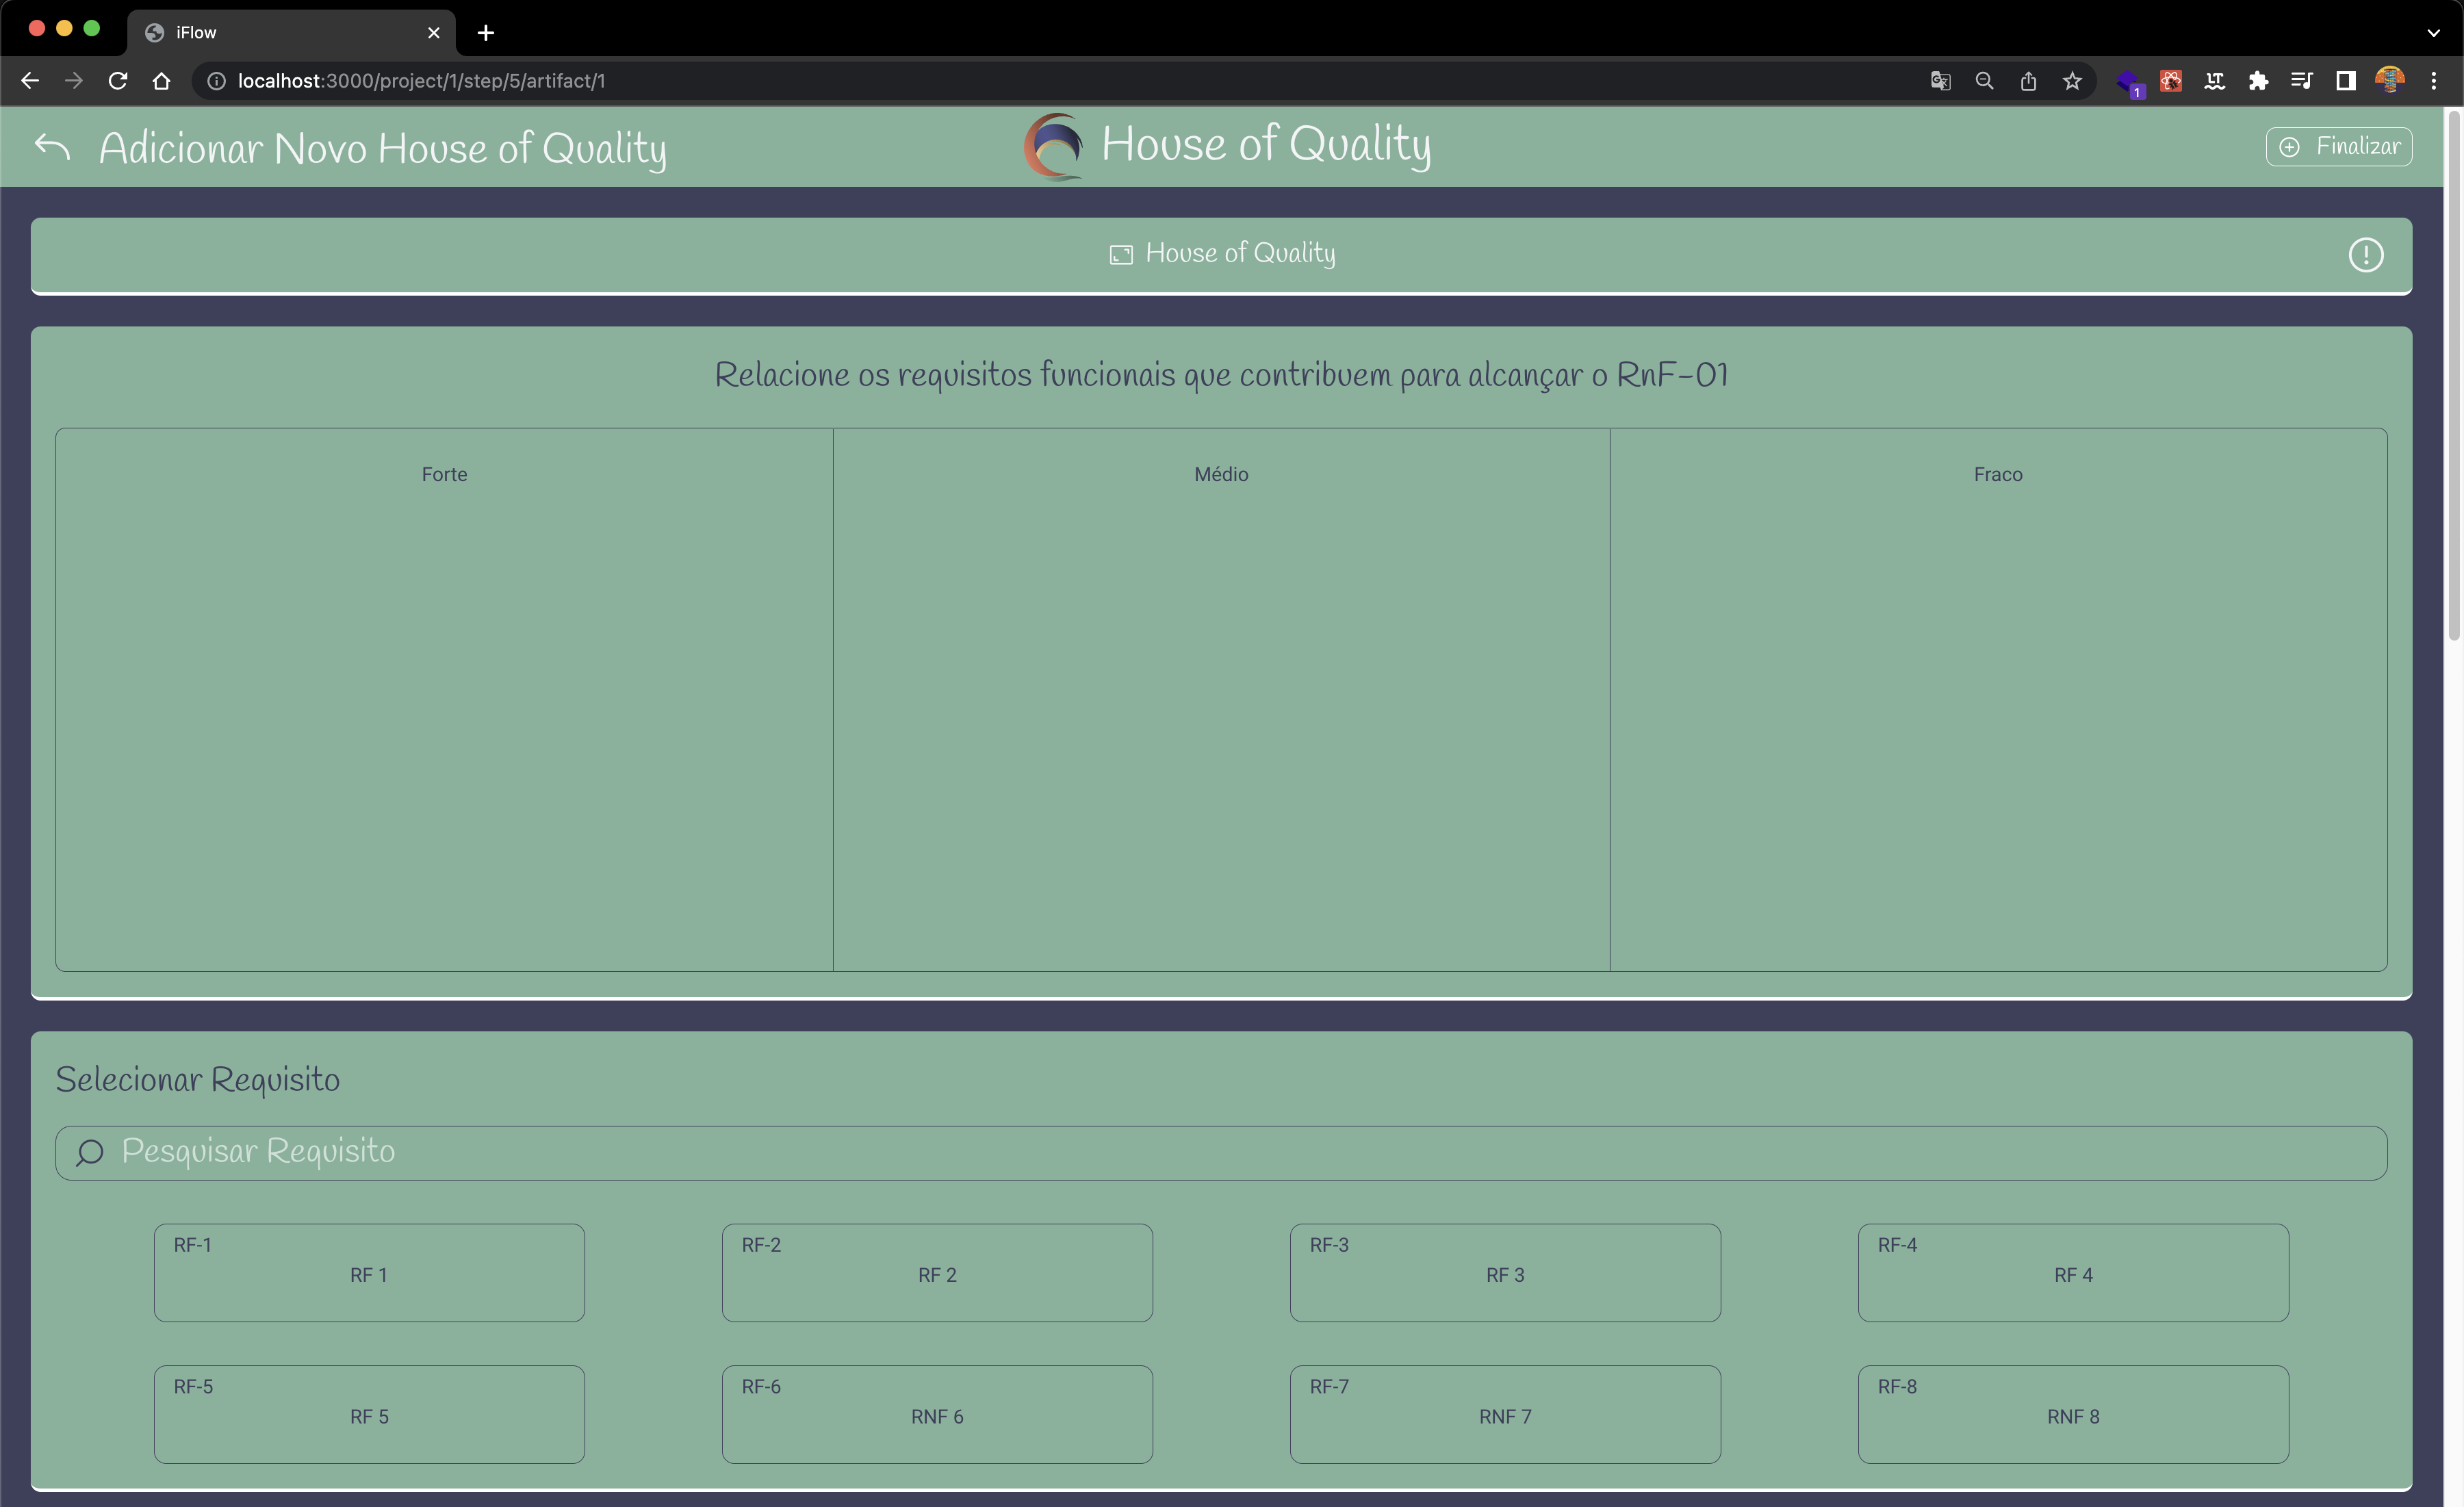
\includegraphics[scale=0.22]{figuras/TelasDesenvolvidas/house-of-quality-implementada.png}
        \legend{Fonte: Autores, 2022.}
    \end{center}
    \end{figure}

\end{itemize}

\subsection{Priorização das funcionalidades do \textit{iFlow}}

\label{sec:priorizacao_iFlow}

A Engenharia de Requisitos trata de uma parte vital do processo de desenvolvimento de um \textit{software}. Portanto, representa uma etapa minuciosa e meticulosa que visa concretizar desejos, pensamentos, demandas e requisitos concretos que possam ser codificados. Entretanto, representa também uma etapa que demanda tempo considerável para a sua correta execução.

Sabendo disso, para viabilizar as etapas do processo, e ainda obter um Produto Mínimo Viável em sua versão preliminar, o principal diferencial da ferramenta, foram priorizadas as funcionalidades mínimas para gerar insumos para tal feito, sendo elas:

\begin{itemize}
    \item Toda a parte de geração de artefatos, tanto na pré-rastreabilidade quanto na elicitação, para que possibilitasse a geração de requisitos mais concisos e completos;
    \item Todas as funcionalidades relacionadas à geração do \textit{Backlog} e do \textit{NFR}, para que os requisitos fossem modelados e amadurecidos para serem usados posteriormente;
    \item A funcionalidade da \textit{House of Quality} para poder viabilizar a modelagem dos requisitos como um grafo, conferindo insumos para a geração do Produto Mínimo Viável em sua versão preliminar;
    \item O algoritmo de menor caminho necessário para viabilizar a geração do Produto Mínimo Viável em sua versão preliminar, e
    \item A parte do gerenciamento de usuário que viabilizasse controle, organização e segurança de tudo que está sendo desenvolvido na ferramenta.
\end{itemize}

Vale ressaltar que, outro ponto que guiou o desenvolvimento da ferramenta, foi o uso das melhores práticas de padrões e desenho de projeto da Engenharia de \textit{Software}, para que fossem gerados códigos de qualidade, não apenas com o intuito de fazer a aplicação, mas de gerar algo que possa ser aperfeiçoado em trabalhos futuros, servindo de base de código para outros trabalhos.

\subsection{Ajustes de Escopo}
\label{sub:corte_de_escopo}

A partir do exposto na Seção \ref{sec:priorizacao_iFlow}, e conferindo ajustes no escopo do desenvolvimento da ferramenta, algumas \textit{features} e \textit{user stories} não foram concluídas. Isso era esperado, dado que o escopo do projeto era abrangente, e precisava ser ajustado para os prazos de um Trabalho de Conclusão de Curso. Entretanto, optou-se por especificar, desde o começo, algo mais refinado e completo, visando facilitar evoluções futuras da ferramenta \textit{iFlow}, e procurando incorporar muitos dos aspectos, estudados na literatura especializada, e que conferem uma visão bastante adequada às atividades da Engenharia de Requisitos. Seguem as \textit{features} e \textit{user stories} não concluídas:

\begin{enumerate}
    \item \textbf{US012}: funcionalidade de \textit{hiperlinkagem} dos léxicos em textos e definições presentes na ferramenta;
    \item \textbf{FE004}: \textit{feature} relacionada à etapa de verificação;
    \item \textbf{FE008}: \textit{feature} relacionado ao escopo de edição das informações da conta de usuário, e
    \item \textbf{US030}: funcionalidade de geração de relatórios com base nos artefatos de cada etapa.
\end{enumerate}

Uma visualização mais precisa e descritiva dessas funcionalidades pode ser conferida na Tabela \ref{tab:backlog}.

\subsection{Base de código da Ferramenta \textit{iFlow}}

A base de código da ferramenta \textit{iFlow} pode ser encontrada na plataforma GitHub, na organização do projeto, por meio do link: \citeauthoronline{github_iFlow} (\citeyear{github_iFlow}).

Há muitos aspectos interessantes, em termos de implementação da Ferramenta \textit{iFlow}. Entretanto, cabe um olhar mais aprofundado  em dois pontos:

\definecolor{codegray}{rgb}{0.5,0.5,0.5}
\definecolor{codepurple}{rgb}{0.58,0,0.82}
\definecolor{backcolour}{rgb}{0.95,0.95,0.92}
\begin{enumerate}
    \item Implementação de telas complexas, tal como ocorre para o caso da tela do \textit{Backlog} do Produto, pelo fato de existir uma funcionalidade de \textit{Drag and Drop} para os requisitos em tela, conferindo maior usabilidade para o usuário na hora de construir este artefato.

    \label{codigo:backlog}
    
    \lstinputlisting[language=Java,caption=\textit{Drag and Drop} na tela do \textit{Backlog} do Produto]{figuras/Codigos/draganddrop.tsx}
        
    Um código similar também foi utilizado na tela da \textit{House of Quality}, já que ambas as telas possuem a funcionalidade de \textit{Drag and Drop}. O código completo encontra-se no seguinte link: \citeauthoronline{tela_backlog_iflow} (\citeyear{tela_backlog_iflow}). Esse \textit{script} tem o objetivo de deixar os \textit{cards} referentes aos requisitos funcionais como arrastáveis, para facilitar a construção do \textit{Backlog} do Produto.
    
    \item Geração do Produto Mínimo Viável, em sua forma preliminar, por meio da  \textit{House of Quality} (Seção \ref{sec:house_of_quality}) com uso de \textit{grafos} (Seção \ref{sec:grafos}) e do algoritmo de menor caminho. A modelagem do grafo deu-se da seguinte forma:
    
    \begin{enumerate}
        \item Cada um dos requisitos, amadurecidos na etapa de \textit{modelagem} (Seção \ref{sec:modelagem_proposta}), funcionais, categorizados como \textit{user story}, e não funcionais, do último nível do NFR, representa um vértice do grafo;
        \item As arestas são bidirecionais, definidas na etapa de desenvolvimento da \textit{House of Quality}, de forma que o usuário indica o tipo de relação: Forte, considerado peso 2; Média, considerando peso 5; e Fraca, considerando peso 9;
        \item Todas as relações indicadas pelo usuário são salvas no banco de dados por meio do relacionamento gerado na tabela de \textbf{House of Quality}, como pode ser visto na Figura \ref{fig:diagrama_logico}, e
        \item O algoritmo de menor caminho de \textbf{Dijkstra}, sendo uma biblioteca disponibilizada pelo \textit{NPM}, é rodado de forma que o começo e o fim do algoritmo são definidos a partir da combinação sem repetição entre os 3 requisitos não funcionais obtidos no NFR.
    \end{enumerate}
    
    O código responsável pelo cálculo do menor caminho, implementado no \textit{backend}, pode ser visto na seção a seguir. Vale ressaltar que o mesmo foi encapsulado com um \textit{Provider}, ou seja, ele possui uma interface comum que pode ser usada para implementar outro tipo de algoritmo de menor caminho, como, por exemplo, Floyd-Warshall. Este pode ser facilmente plugado na rota responsável por retornar esse resultado para o \textit{frontend}.
    
    \lstinputlisting[language=Java,caption={Algoritmo do Menor Caminho (Dijkstra)}]{figuras/Codigos/DijkstraProvider.ts}

\end{enumerate}

\section{Resumo do Capítulo}

\label{sec:resumo_proposta}
Neste capítulo, foi apresentado o \textit{iFlow}, que consiste em uma ferramenta que possibilita a semiautomatização, conferindo apoio nos processos da Engenharia de Requisitos. Para isso, foi apresentada a contextualização do \textit{iFlow}; uma seção abordando a ferramenta \textit{iFlow} e seus principais pontos; a arquitetura da solução, com detalhamento dos componentes presentes na mesma; a identidade visual da ferramenta e os diagramas do \textit{iFlow}, sendo o Diagrama de Banco de Dados e o Diagrama de Pacotes.

Além disso, foram mostradas as telas mais relevantes do Protótipo de Alta Fidelidade, Backlog do Produto, e as telas desenvolvidas em sua versão final. Por fim, há uma breve ponderação sobre o escopo da ferramenta.